\documentclass[11pt, oneside,titlepage]{article}   	% use "amsart" instead of "article" for AMSLaTeX format
\usepackage[margin=1in]{geometry}                		% See geometry.pdf to learn the layout options. There are lots.
\geometry{letterpaper}                   		% ... or a4paper or a5paper or ... 
%\geometry{landscape}                		% Activate for rotated page geometry
\usepackage[parfill]{parskip}    		% Activate to begin paragraphs with an empty line rather than an indent
\usepackage{graphicx}				% Use pdf, png, jpg, or eps§ with pdflatex; use eps in DVI mode
								% TeX will automatically convert eps --> pdf in pdflatex		
\usepackage{amssymb}
\usepackage{etoolbox}
\usepackage{lipsum}
\usepackage{caption}
\usepackage{subcaption}
\usepackage{float}
\usepackage[all]{nowidow}
\usepackage[hang,flushmargin]{footmisc}

    \AfterEndEnvironment{hangparas}{\addvspace{0.67\baselineskip}}
    \usepackage[notquote]{hanging}


\title{What (and Whom) to Avoid On the Roads}
\author{Desmond Cole - \\
Teerth Patel - \\ 
Yunbin Peng}

\begin{document}
\interfootnotelinepenalty=10000
\maketitle
\section*{Introduction}
\subsection*{Executive Summary}
In the United States, approximately 35-40,000 people die in vehicle-related incidents every year. The fatality rate declined significantly in the second half of the 20th century, and continued to decline in the 21st, however the decline has plateaued in recent years, to a rate of just over 1 death per 100 million vehicle miles traveled (VMT). Understanding and tackling the problem of crash fatalities has motivated considerable improvements and investments in vehicle design, road design, and our knowledge of human motor skills and reaction times. \\ 

With this analysis, we set out to survey the distribution of vehicle-related fatalities across geography and time, and explore a number of driver-specific characteristics to assess dominant contributors to the incidence and extent of vehicle-related deaths. We use this analysis to develop a limited profile of the circumstances associated with traffic fatalities, and of things to avoid if you're considering taking a drive.

\subsection*{Data}
The data used for this analysis are gathered by the National Highway Traffic Safety Administration (NHTSA), a branch of the U.S. Department of Transportation. Traffic fatality data is contained within NHTSA's Fatality Analysis Reporting System (FARS), a nationwide census of various information regarding fatalities occurring in motor vehicle crashes. FARS contains a rich set of different features, with information on crash circumstances, areas of damage, police reports, emergency response times, and vehicle characteristics. We focus specifically on data from 2015 and 2016, and subset a choice set of predictors of interest, paying particular attention to indicators of driver behavior.

\section*{Exploratory Analysis and Visualization}

\subsection*{Geographic Patterns}

\subsection*{Time Trends - Hourly Cycle}
At the national and state level, the cycle of fatal accidents throughout the day is fairly consistent. The below plot shows aggregate fatal accidents per thousand vehicles per hour for the United States, between 2015 and 2016. To account for traffic variability, we weighted the rate of fatal incidents according to hour-by-hour traffic flow allocations estimated by Batterman, et al. (see references). These same flow allocations are used to weight state-by-state hourly trends, under the assumption that state-by-state traffic flow patterns tend to be similar. \\

At the state level, the daily fatal accident cycle is roughly similar. Estimating the overall traffic flow for each state using state-level vehicle registrations, combined with the flow allocations estimated by Batterman, et al. (2015), returns state-level cycles that closely mirror the overall national trend.

\begin{figure}[H]
\centering
\begin{subfigure}{.5\textwidth}
	\centering
	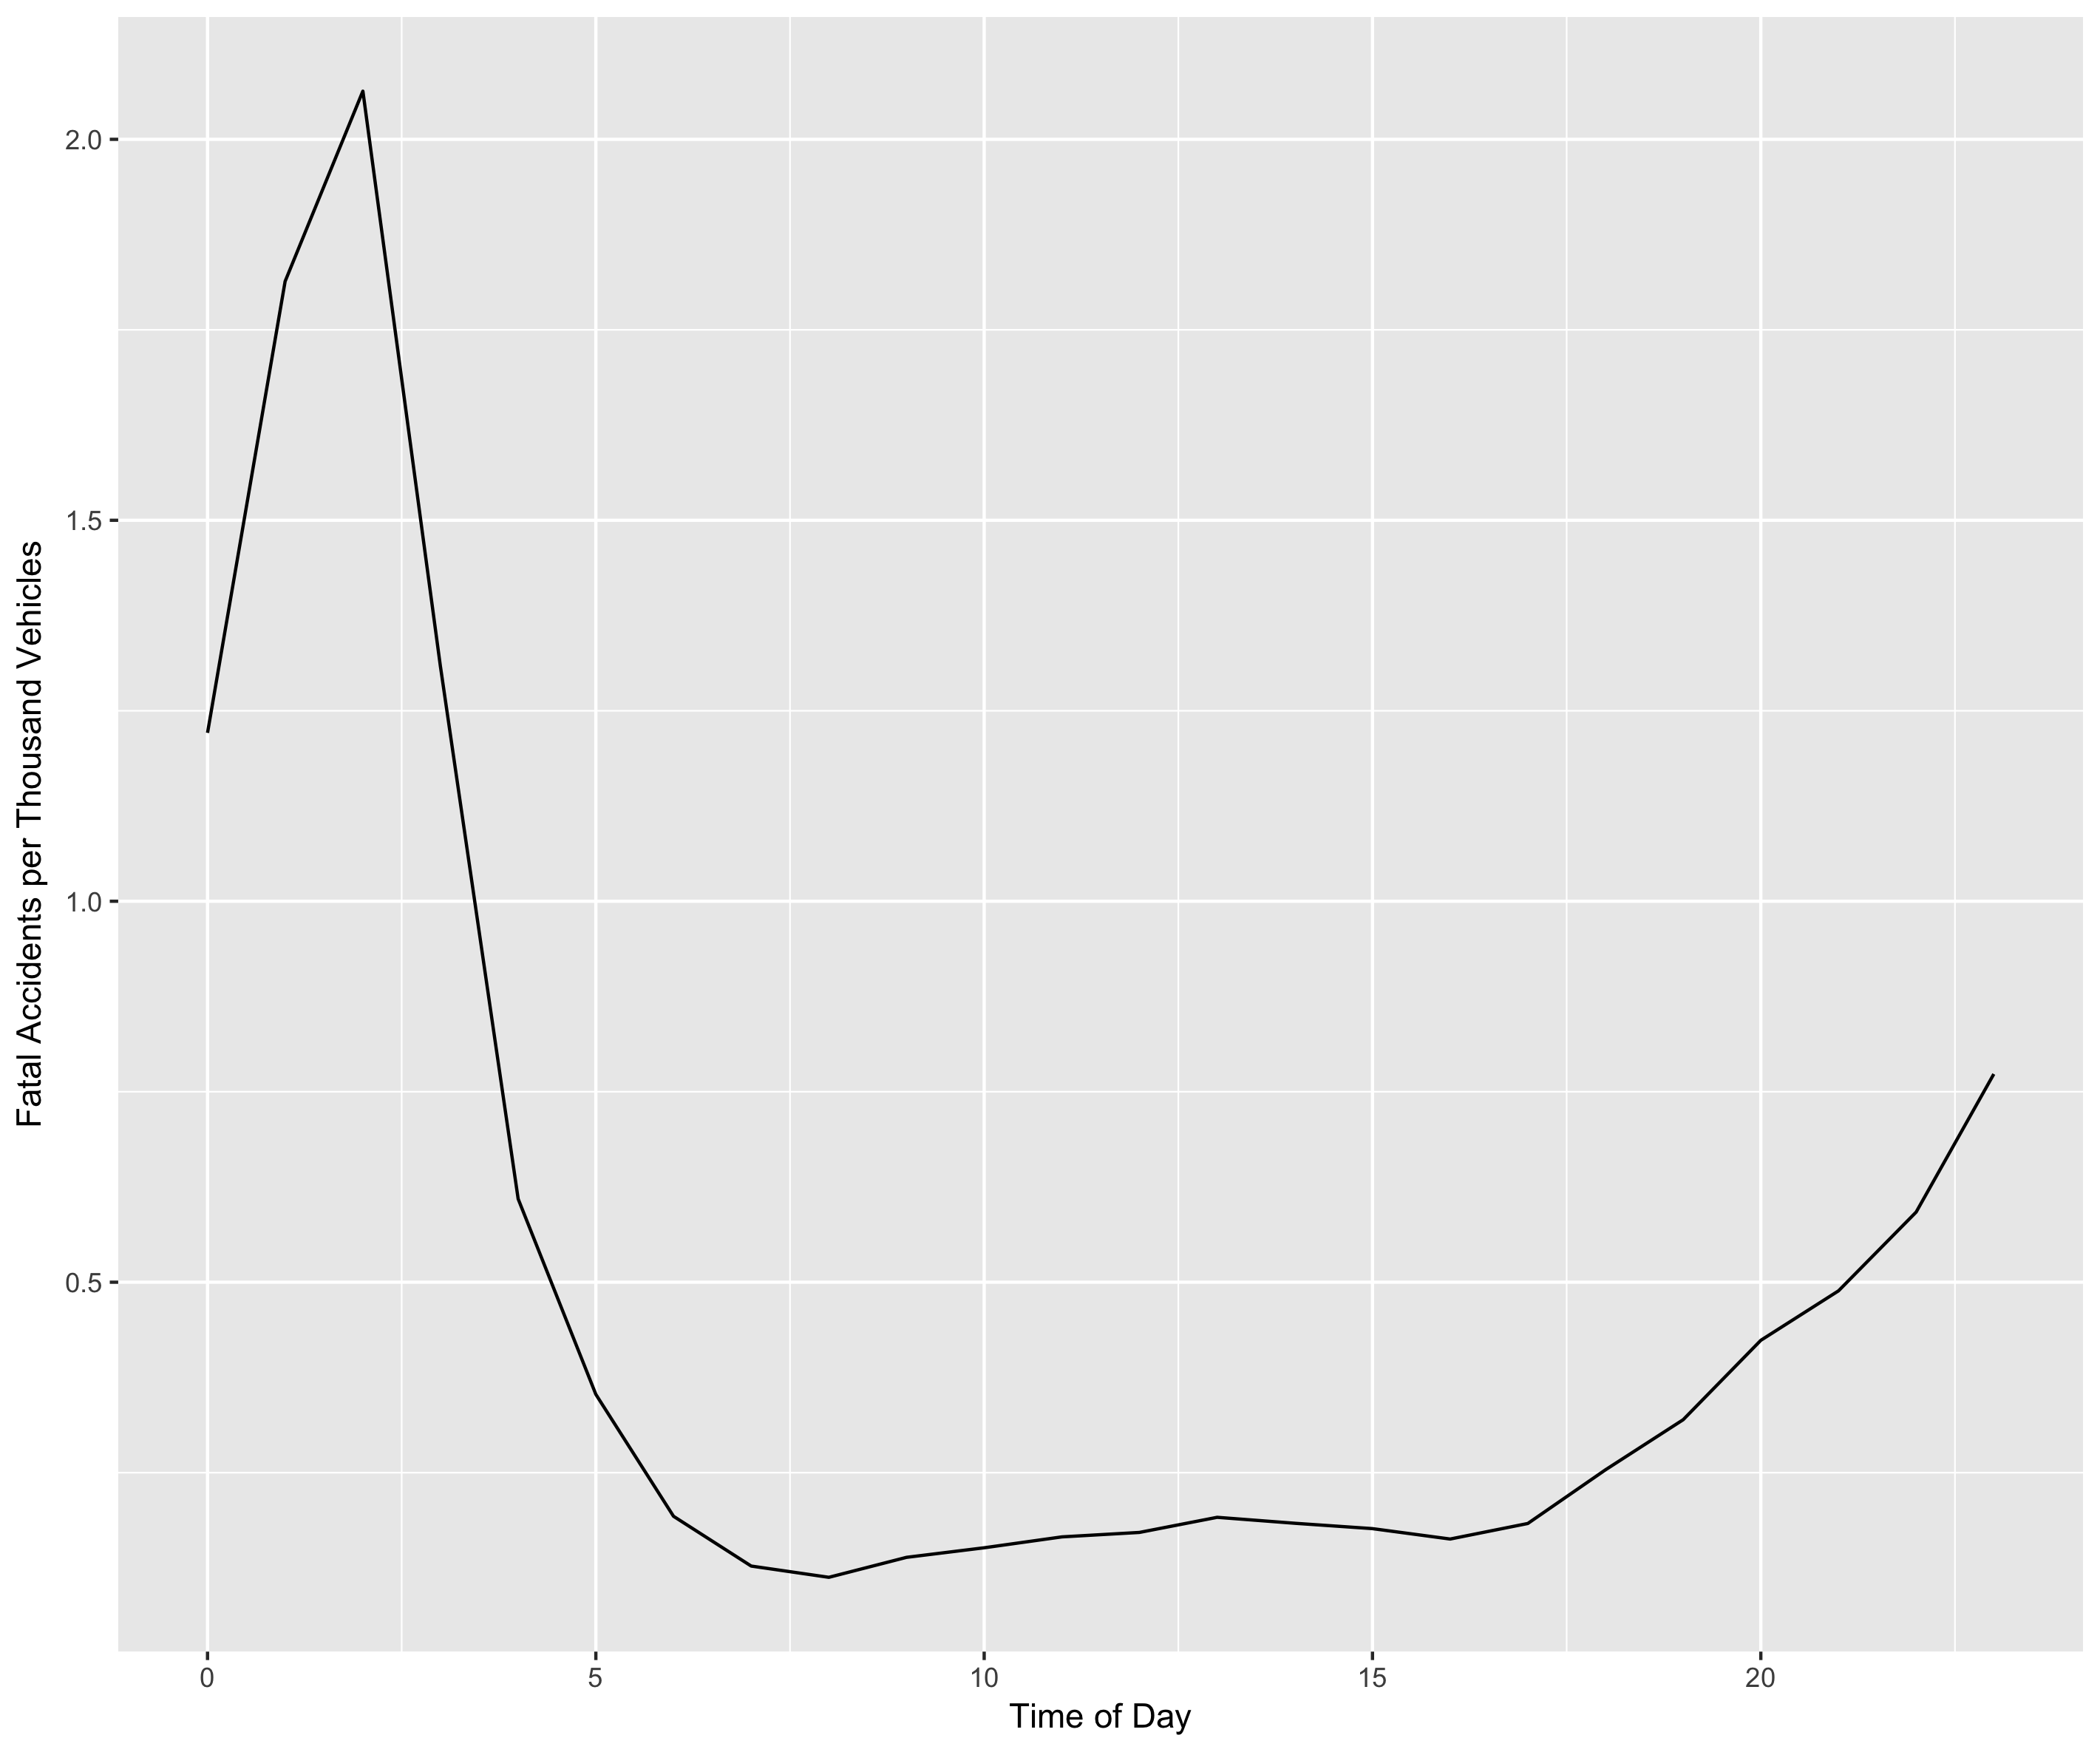
\includegraphics[width=.9\textwidth,height=9cm,keepaspectratio]{WeightedNationalDayTrends.png}
	\label{fig:sub1}
\end{subfigure}%
\begin{subfigure}{.5\textwidth}
  \centering
	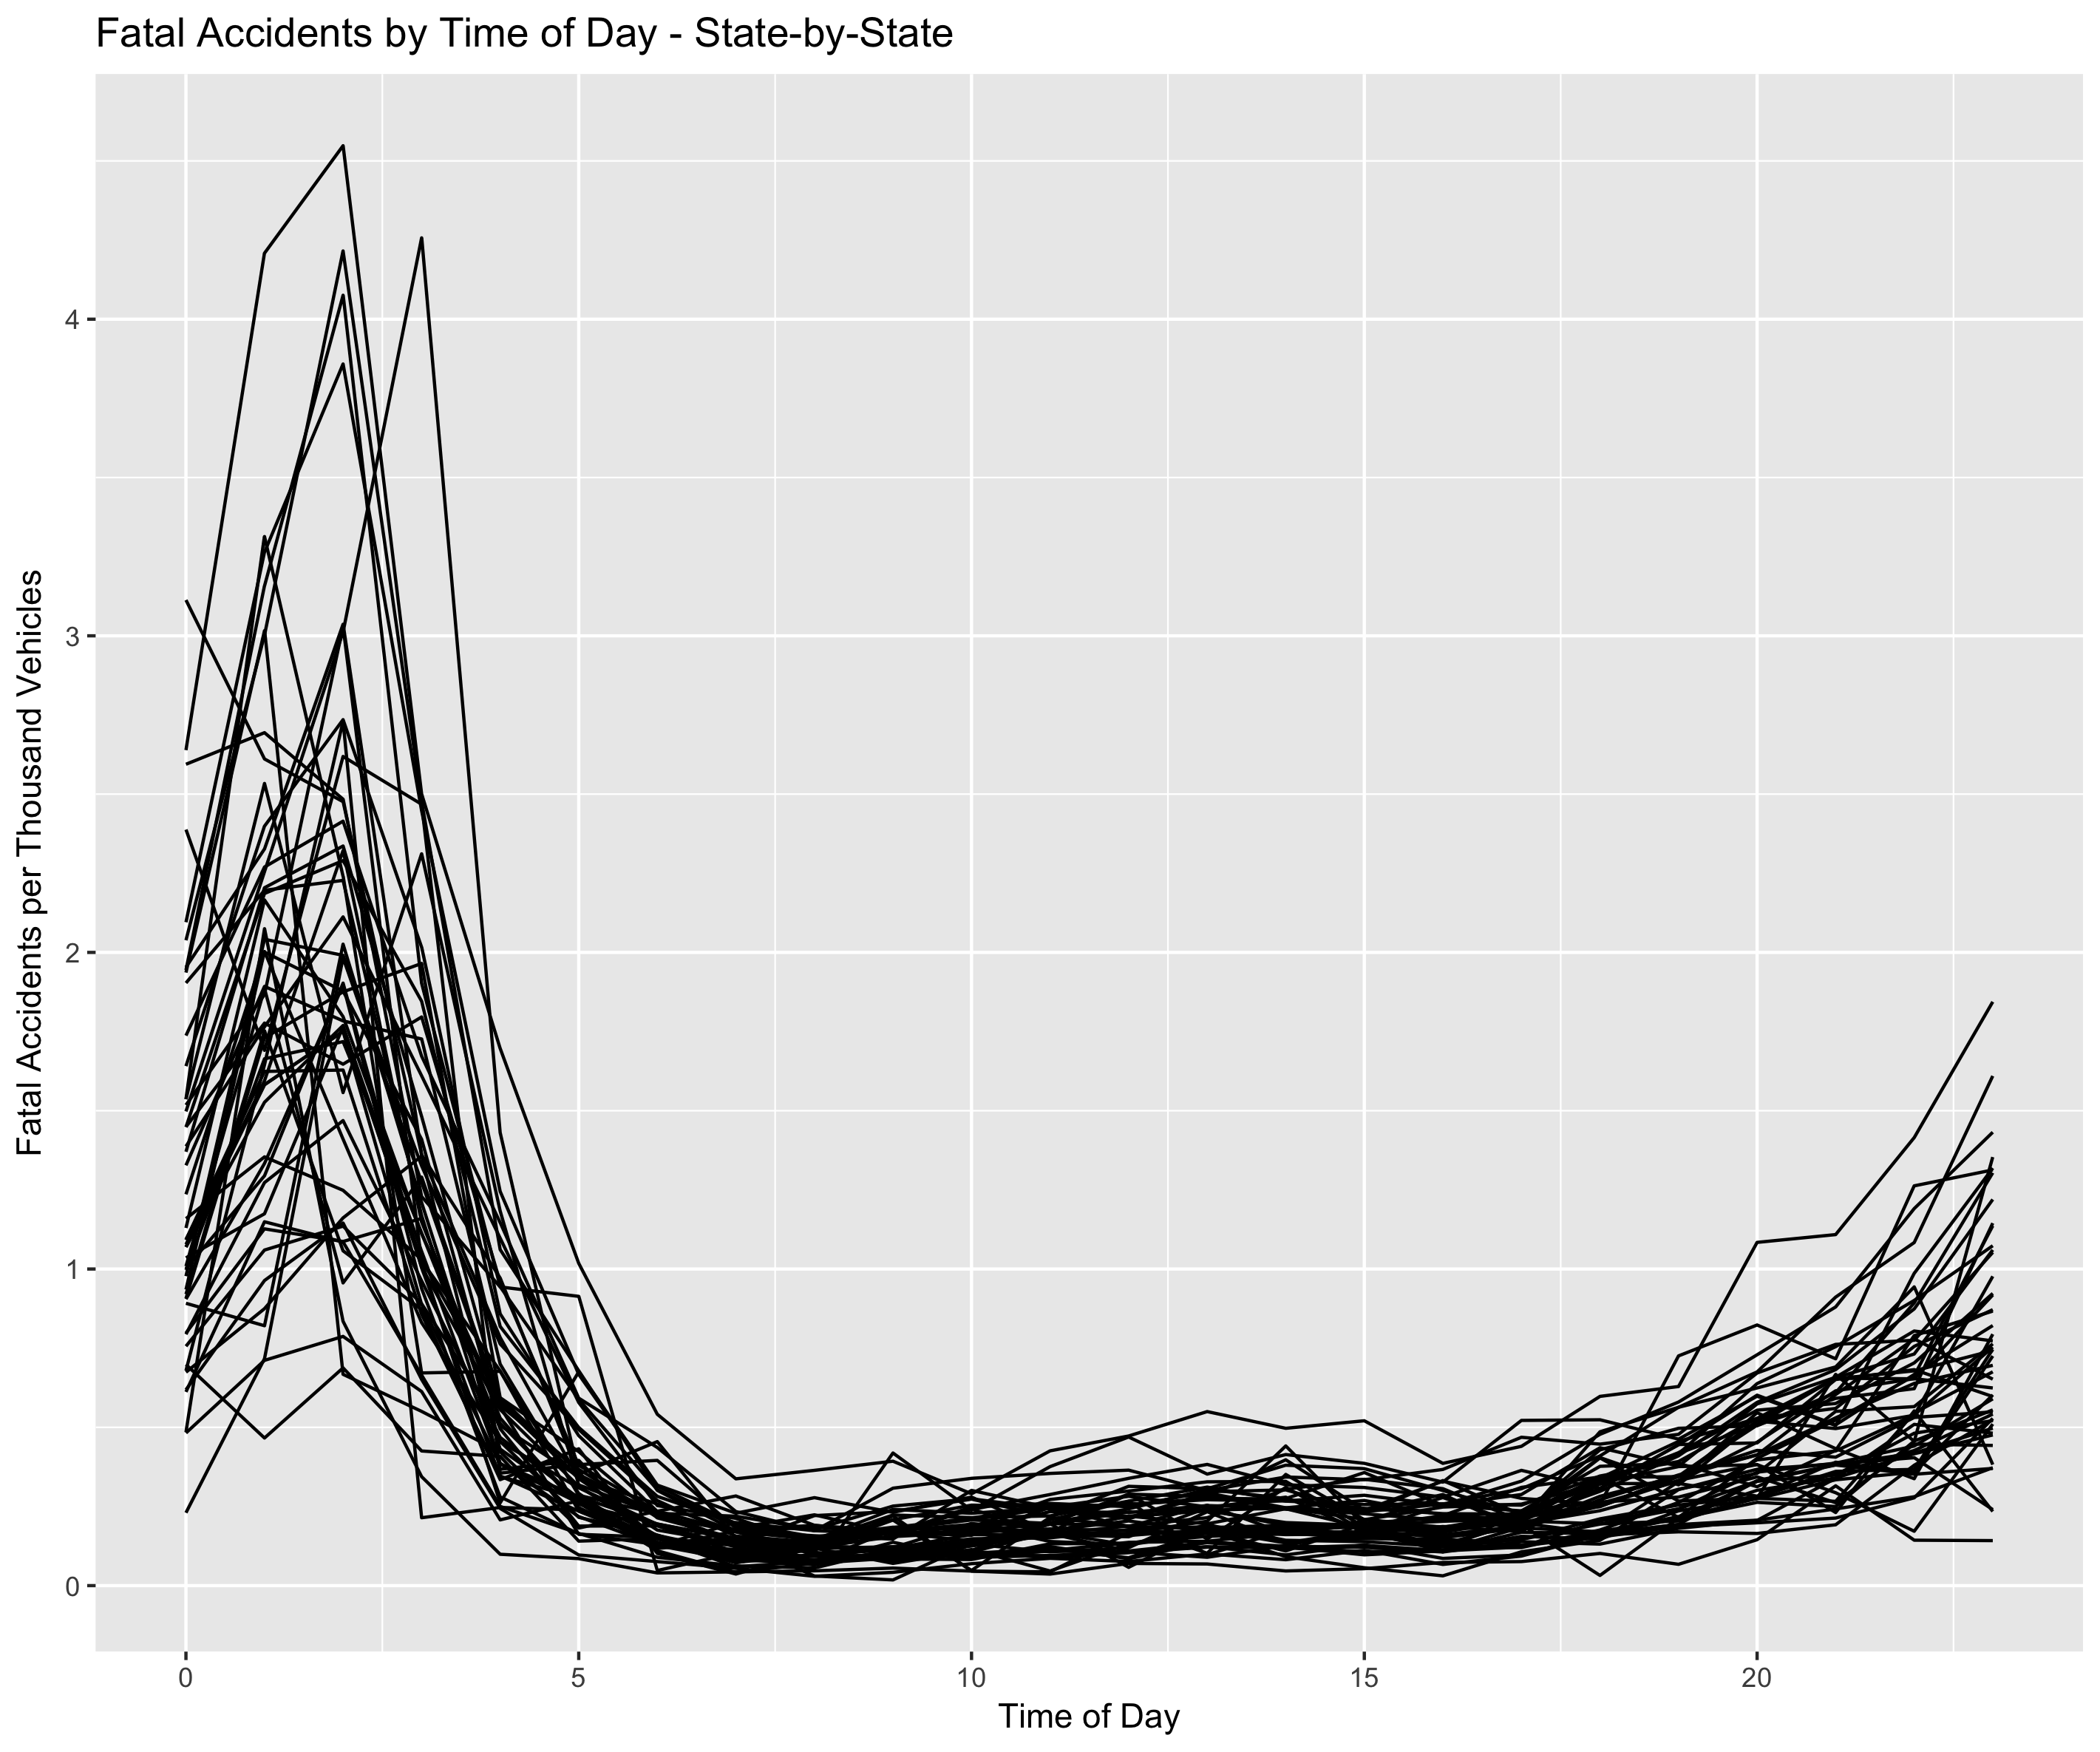
\includegraphics[width=.9\textwidth, height=9cm,keepaspectratio]{WeightedStatePlot.png}
  \label{fig:sub2}
\end{subfigure}
\label{fig:test}
\end{figure}


To tease out potential state-level variation in daily cycles, we used shape-based time series clustering, available in R's dtwclust package. Roughly speaking, this method clusters different time series based on their similarity to different centroids, where a centroid in this case is some typical time trend. Further detail on relevant methods is available in work by Gravano and Paparrizos (2015). Testing different numbers of clusters yielded little overall diversity in terms of performance. A plot of results obtained using 2 clusters is below.\footnote{Across multiple iterations, a 2-cluster separation tends to yield the best performance. For reference in the Validity Index table, optimal clustering will minimize the Silhouette (``Sil"), Davies-Bouldin (``DB" and ``DBstar") indices, and maximize the Dunn index (``D"), Calinski-Harabasz index (``CH"), and Score Function (``SF"). 2 clusters were chosen to be optimal on this basis.} There is little indication of significant variation across clusters, and the clustering results (and performance statistics, shown in the below table) are highly sensitive to initial randomization. 

\begin{center}
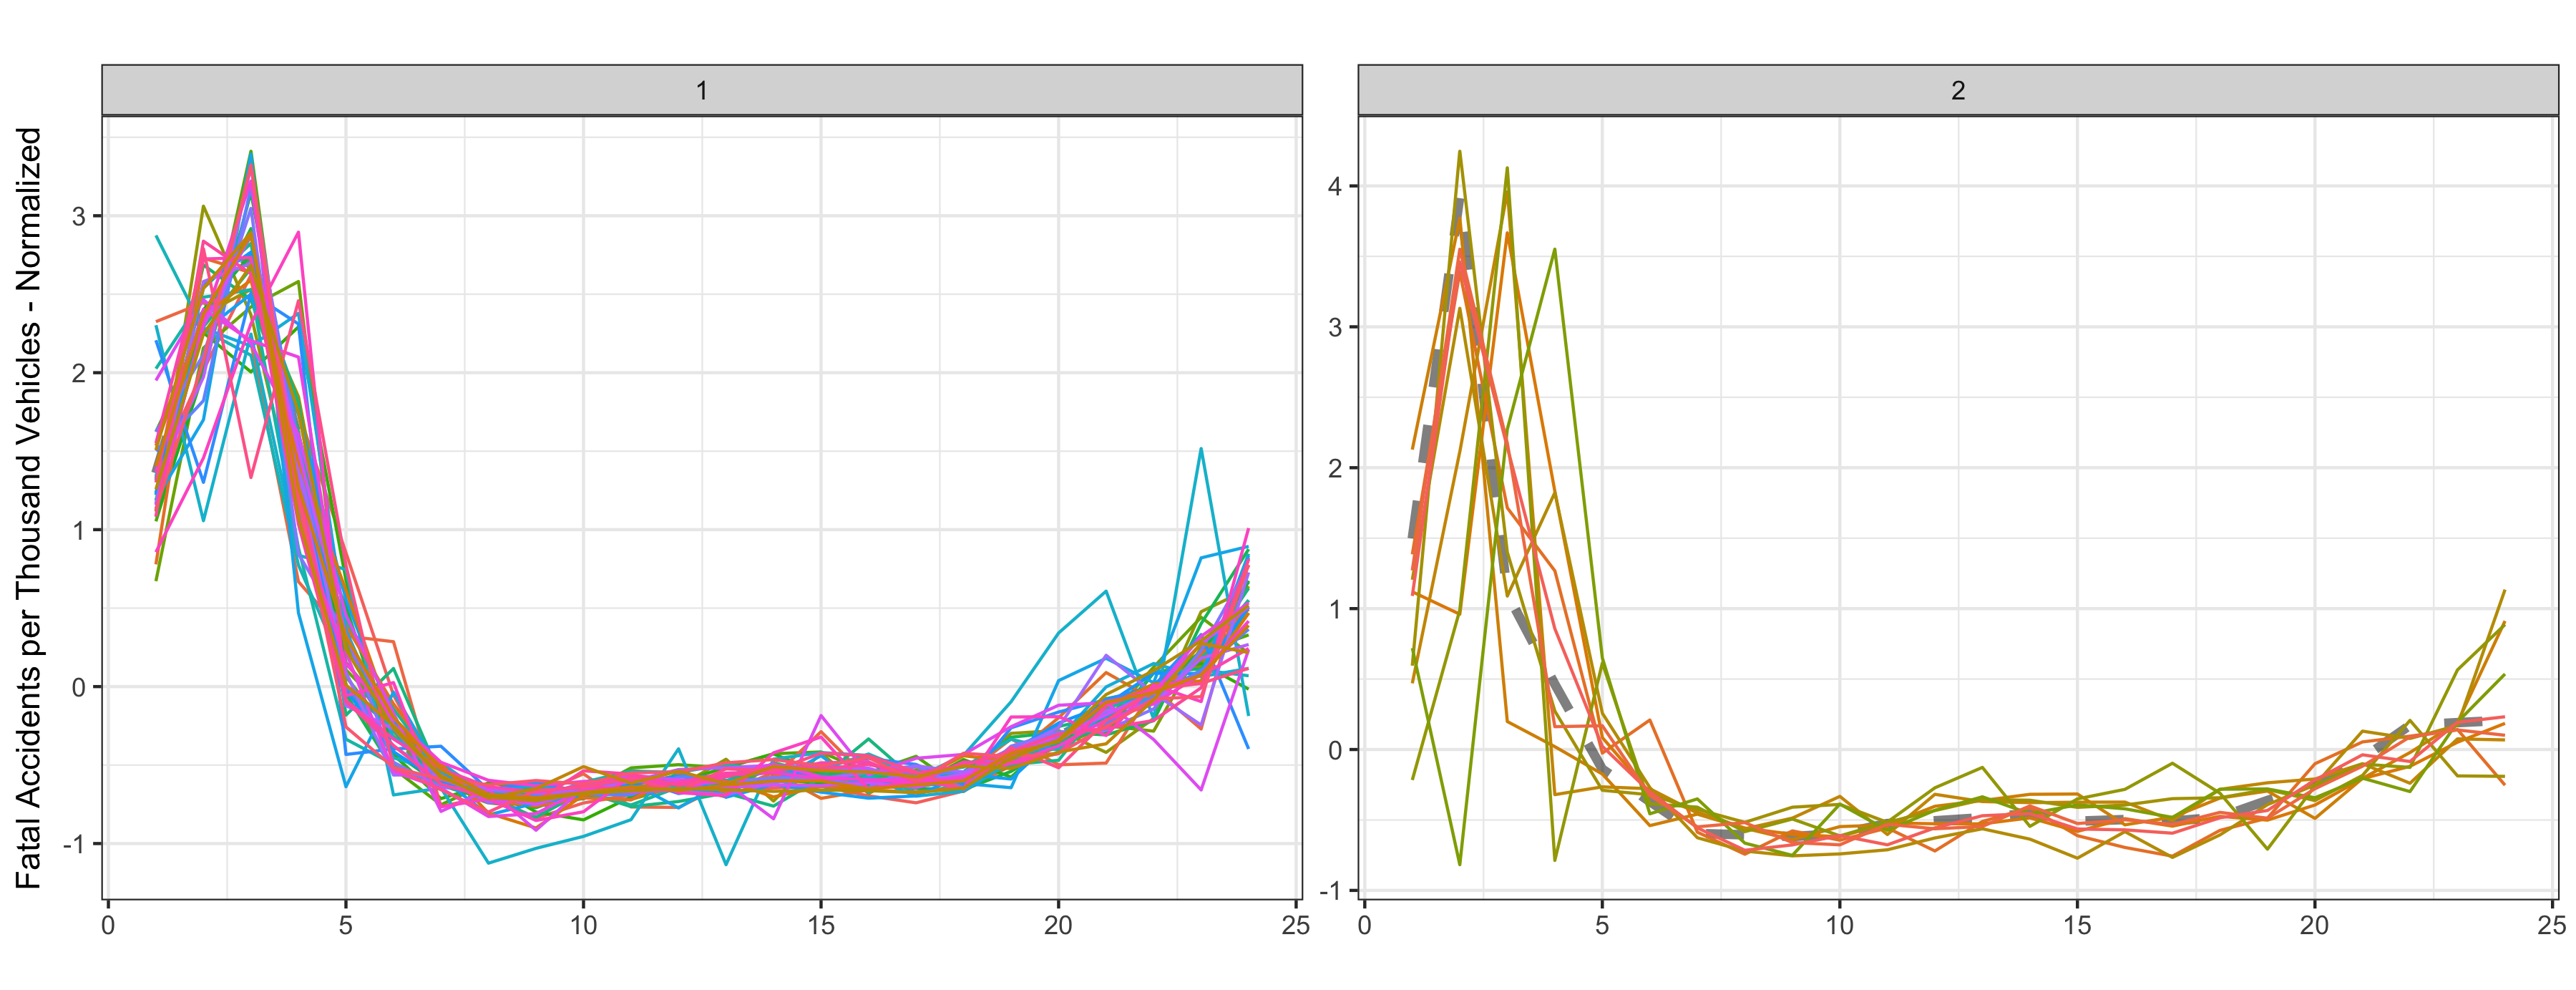
\includegraphics[width=.75\textwidth,height=6cm,keepaspectratio]{StateClusterPlot_Hourly.png}
\end{center}

\begin{table}[H]
\centering
\begin{tabular}{rrrrrrrrr}
  \hline
 & NumClusters & Sil & SF & CH & DB & DBstar & D & COP \\ 
  \hline
1 & 2 & 0.508 & 0.602 & 23.664 & 0.899 & 0.899 & 0.072 & 0.181 \\ 
  2 & 3 & 0.267 & 0.595 & 17.453 & 1.461 & 2.080 & 0.013 & 0.135 \\ 
  3 & 4 & 0.167 & 0.589 & 12.171 & 1.929 & 2.510 & 0.019 & 0.121 \\ 
  4 & 5 & 0.133 & 0.572 & 9.163 & 1.345 & 2.451 & 0.017 & 0.153 \\ 
  5 & 6 & 0.391 & 0.576 & 15.172 & 0.683 & 1.219 & 0.056 & 0.084 \\ 
   \hline
\end{tabular}
\caption{Time Series Cluster Validity Indices (CVIs)} 
\end{table}


\section*{Traffic Fatality Risk Factor Analysis}
We used a mix of classifiers to assess factors relevant to incident fatalities, with a particular focus on driver behavior and vehicle manufacturer. Our analysis begins with an overview of vehicle types/manufacturers, focusing on their relevance within the context of other predictors. We then separately examine different aspects of driver behavior, specifically driver impairment and whether a driver engaged in a hit and run during a given collision. Given that our dataset consists solely of fatal traffic incidents, we choose as a primary output incidents involving more than one fatality.

In several cases, we had to grapple with significant class imbalance. For example, there are far more single-fatality incidents than multi-fatality incidents. As a result, optimal classification in the naive setting without any resampling will occasionally identify all incidents as single-fatality.   

\subsection*{Automakers}

This section explores in some detail different fatality rates for different car types (by automaker, vehicle body, etc.).\footnote{Note that the numbers in this assessment focus on car brands \textit{involved} in fatal incidents. Thus, they do not imply specifically that the vehicle types considered here actually caused death(s), or that the driver(s) of the vehicle(s) themselves died.} For this assessment, we focused on the 15 largest automakers that together produce more than 95\% of the cars and light trucks on American roads. In addition, we subsetted the data to focus specifically on smaller vehicles, excluding commercial vehicles, semi-trucks, etc. \\

The plot below shows a basic ranking of car manufacturers according to the number of fatalities per million vehicles. This is scaled and subsetted according to an approximation of the number and types of vehicles each manufacturer has on the road, but due to a lack of thorough data, it is likely that not all variation simply attributable to manufacturer size and vehicle class has been accounted for. With that said, this plot does suggest that there is meaningful variation across manufacturers in terms of their safety record, with makers such as Subaru and luxury makers such as BMW and Land Rover having significantly less involvement in fatal incidents than carmakers like GM, Ford, and Volvo.
\\
\begin{center}
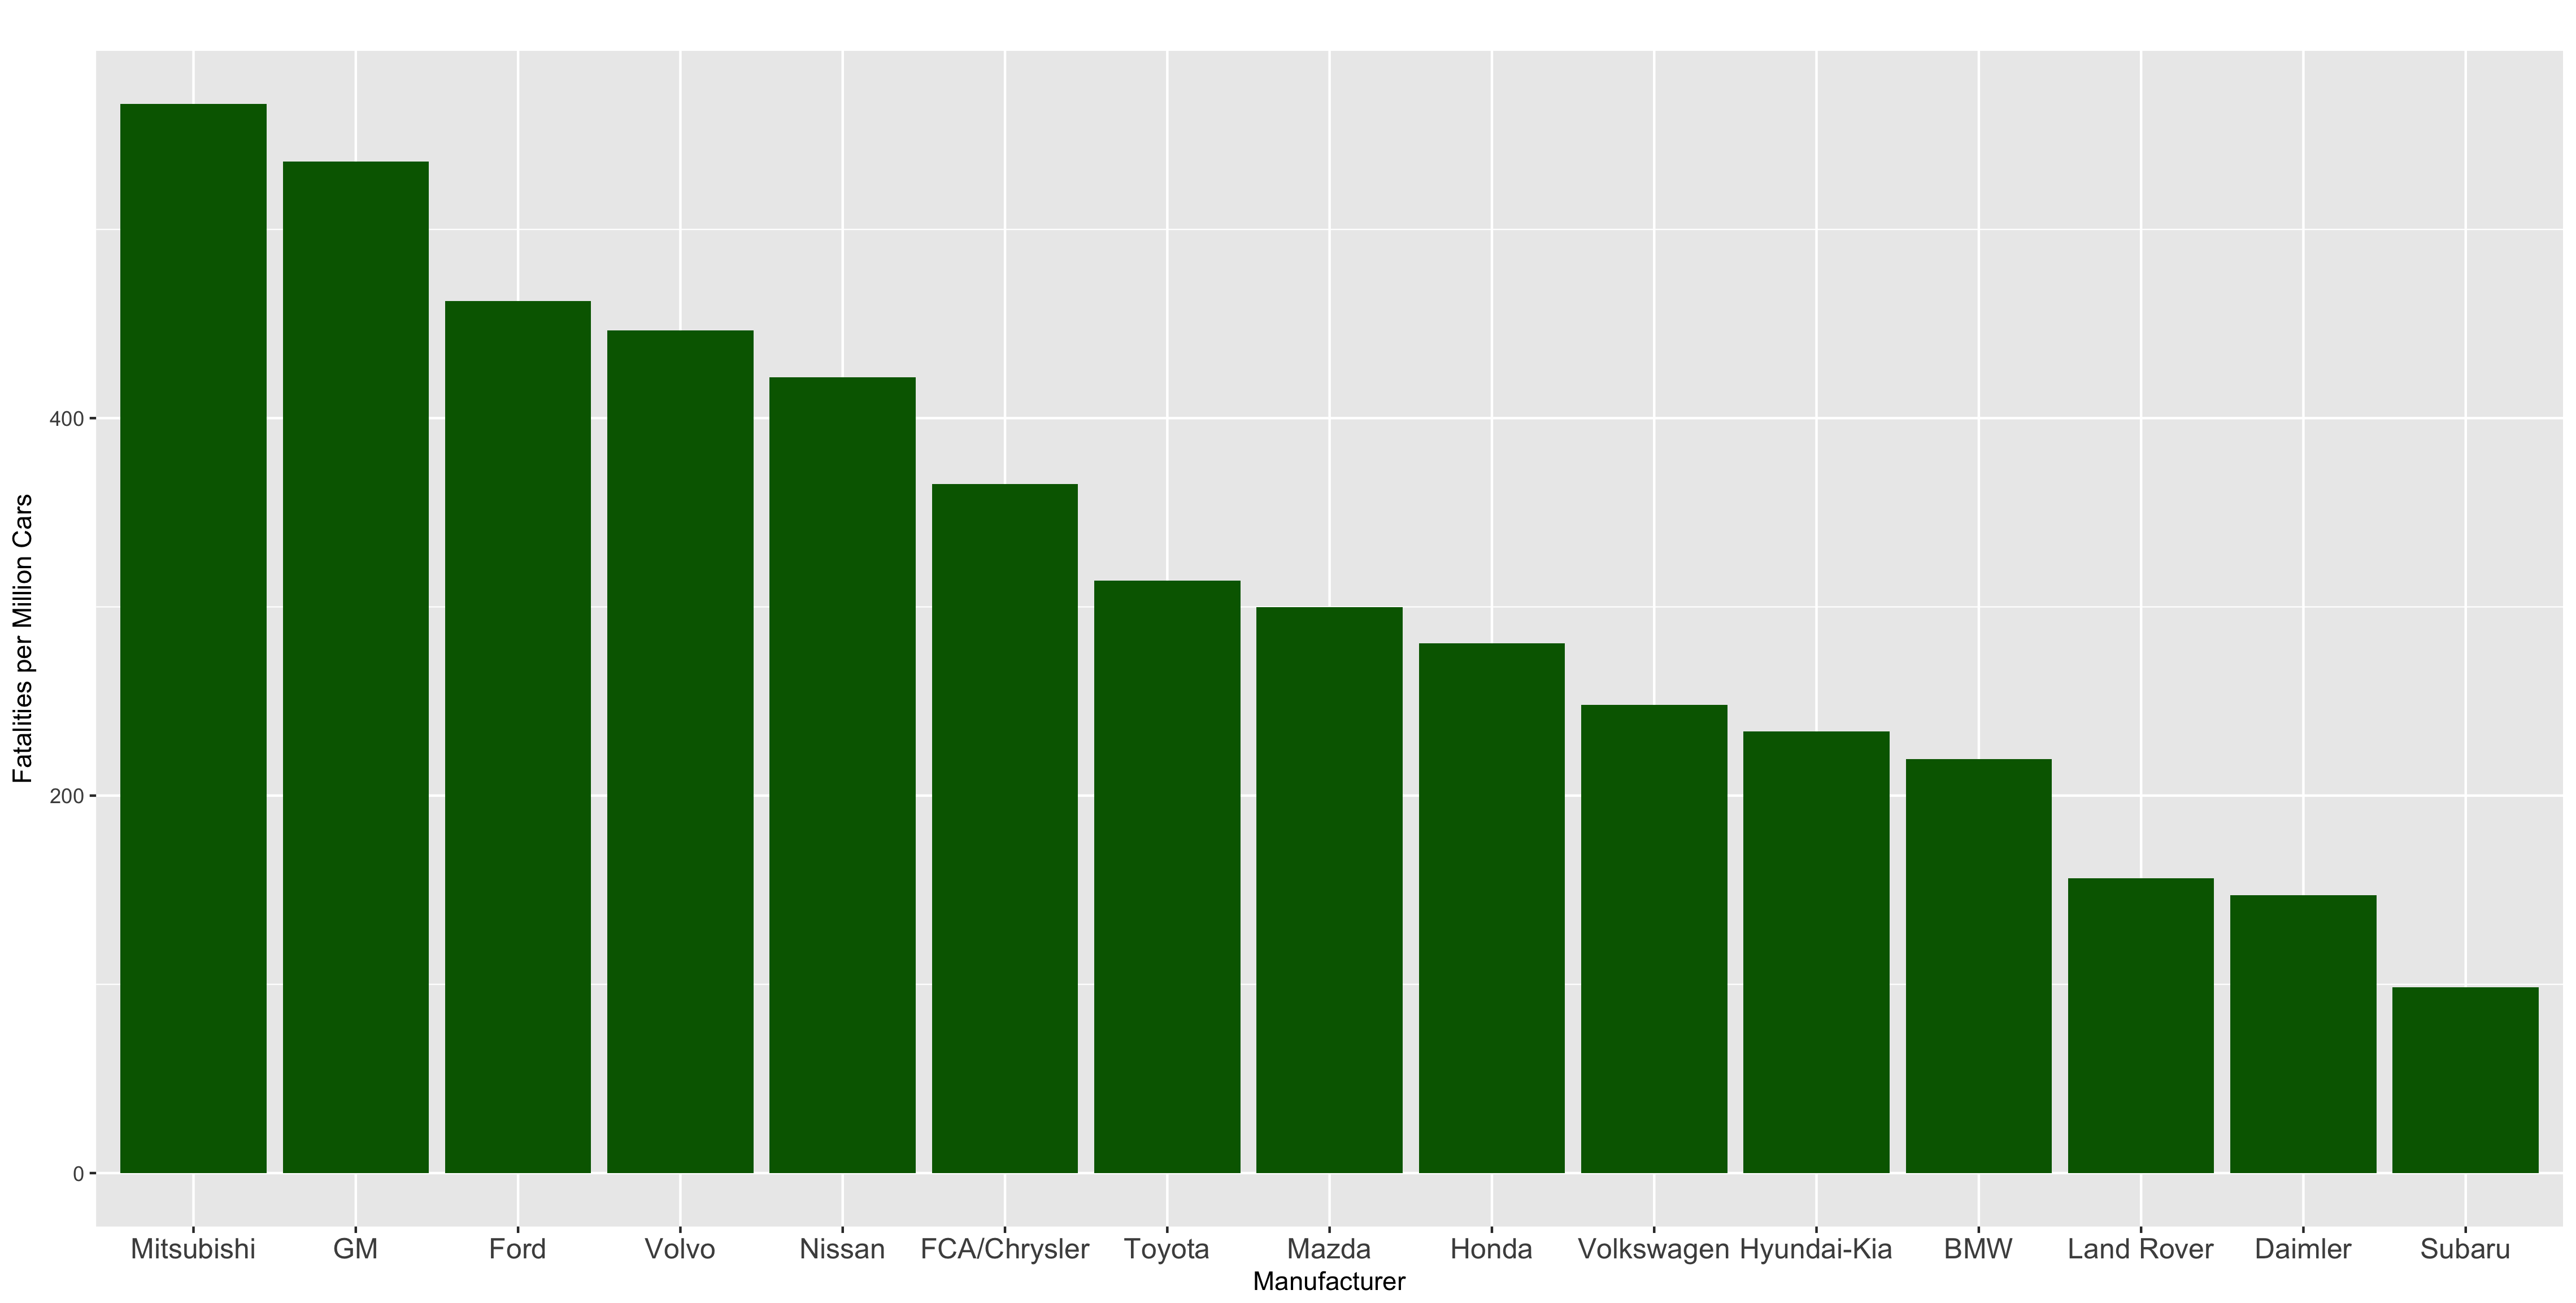
\includegraphics[width=.75\textwidth,height=9cm,keepaspectratio]{ManufacturerRankingPlot.png}
\end{center}

The plot above, although suggestive of meaningful difference across manufacturers, fails to fully account for the various contextual differences across vehicle types which may be unobservable. To further explore the potential relevance of car manufacturer and car type to crash risks, we applied multidimensional scaling to assess visually the differences between vehicles in terms of various driver-specific crash-relevant pieces of information, such as use of restraints, drug/alcohol use, fires, and speeding, with the goal being to assess whether a certain vehicle type or manufacturer predicts the behavior of the vehicle's driver.\\

\begin{figure}[H]
\centering
\begin{subfigure}{.5\textwidth}
	\centering
	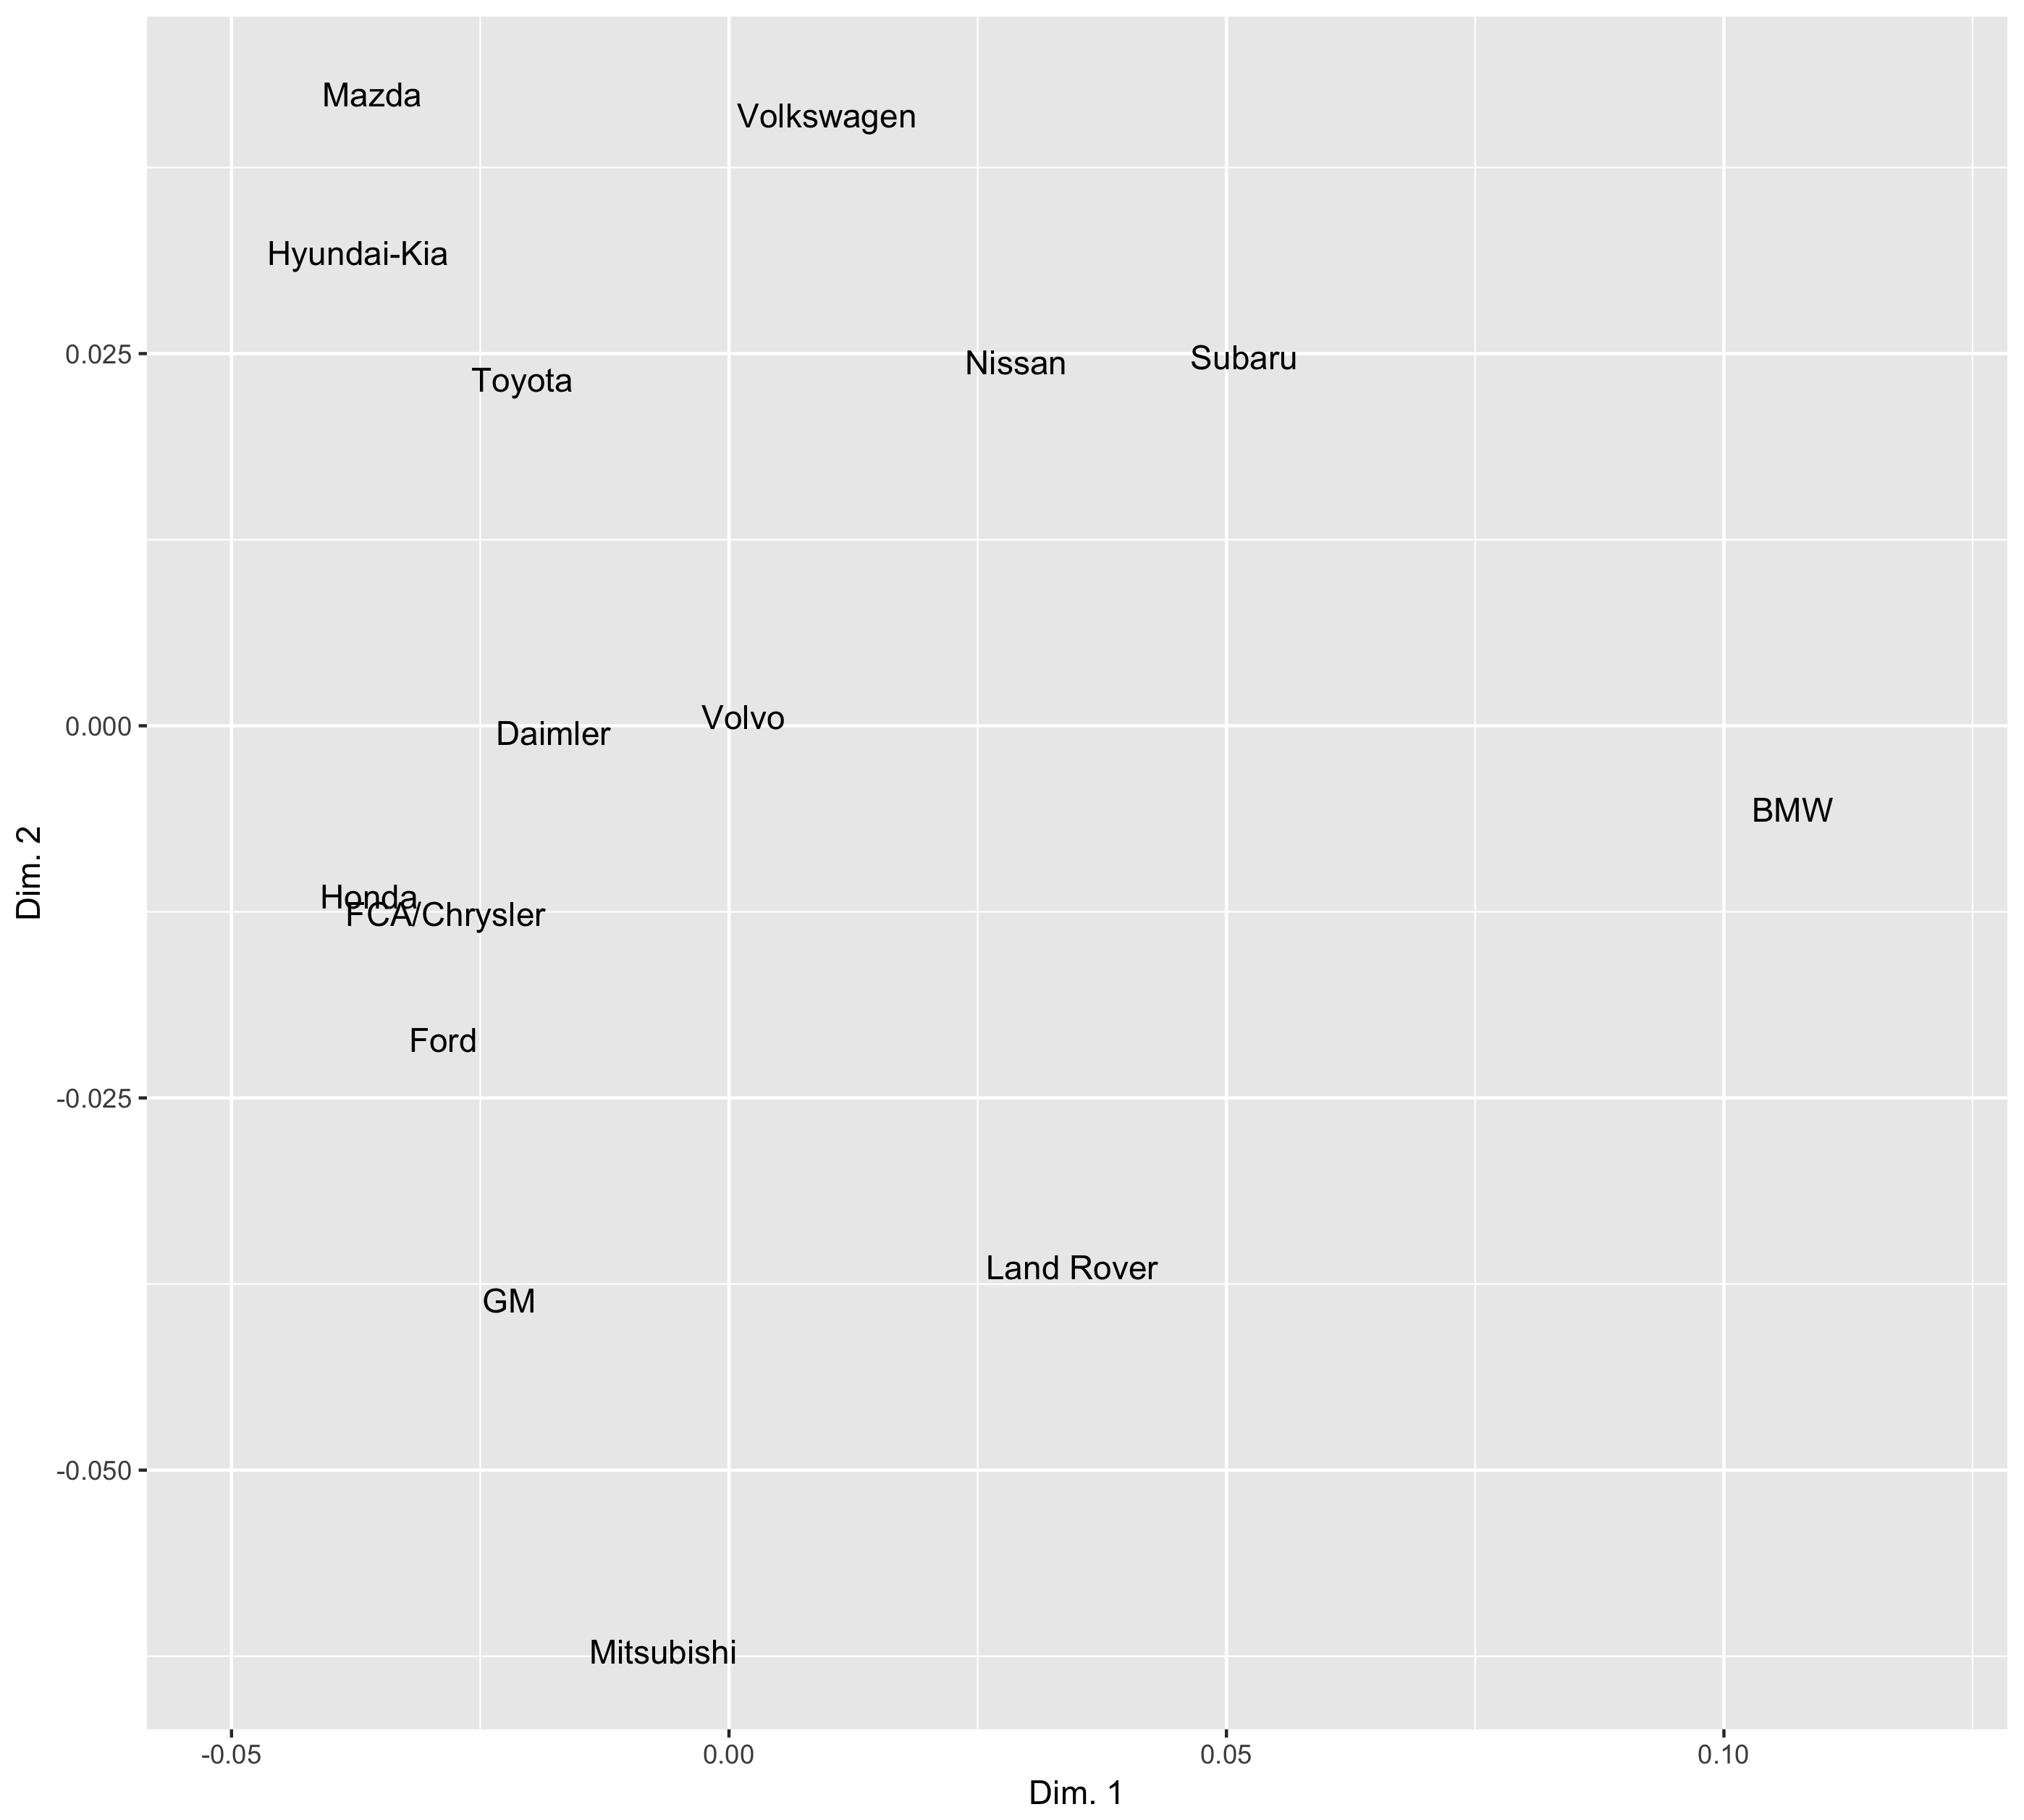
\includegraphics[width=1\linewidth]{ManufacturerMDSPlot.png}
	\caption{Manufacturer MDS}
	\label{fig:sub1}
\end{subfigure}%
\begin{subfigure}{.5\textwidth}
  \centering
  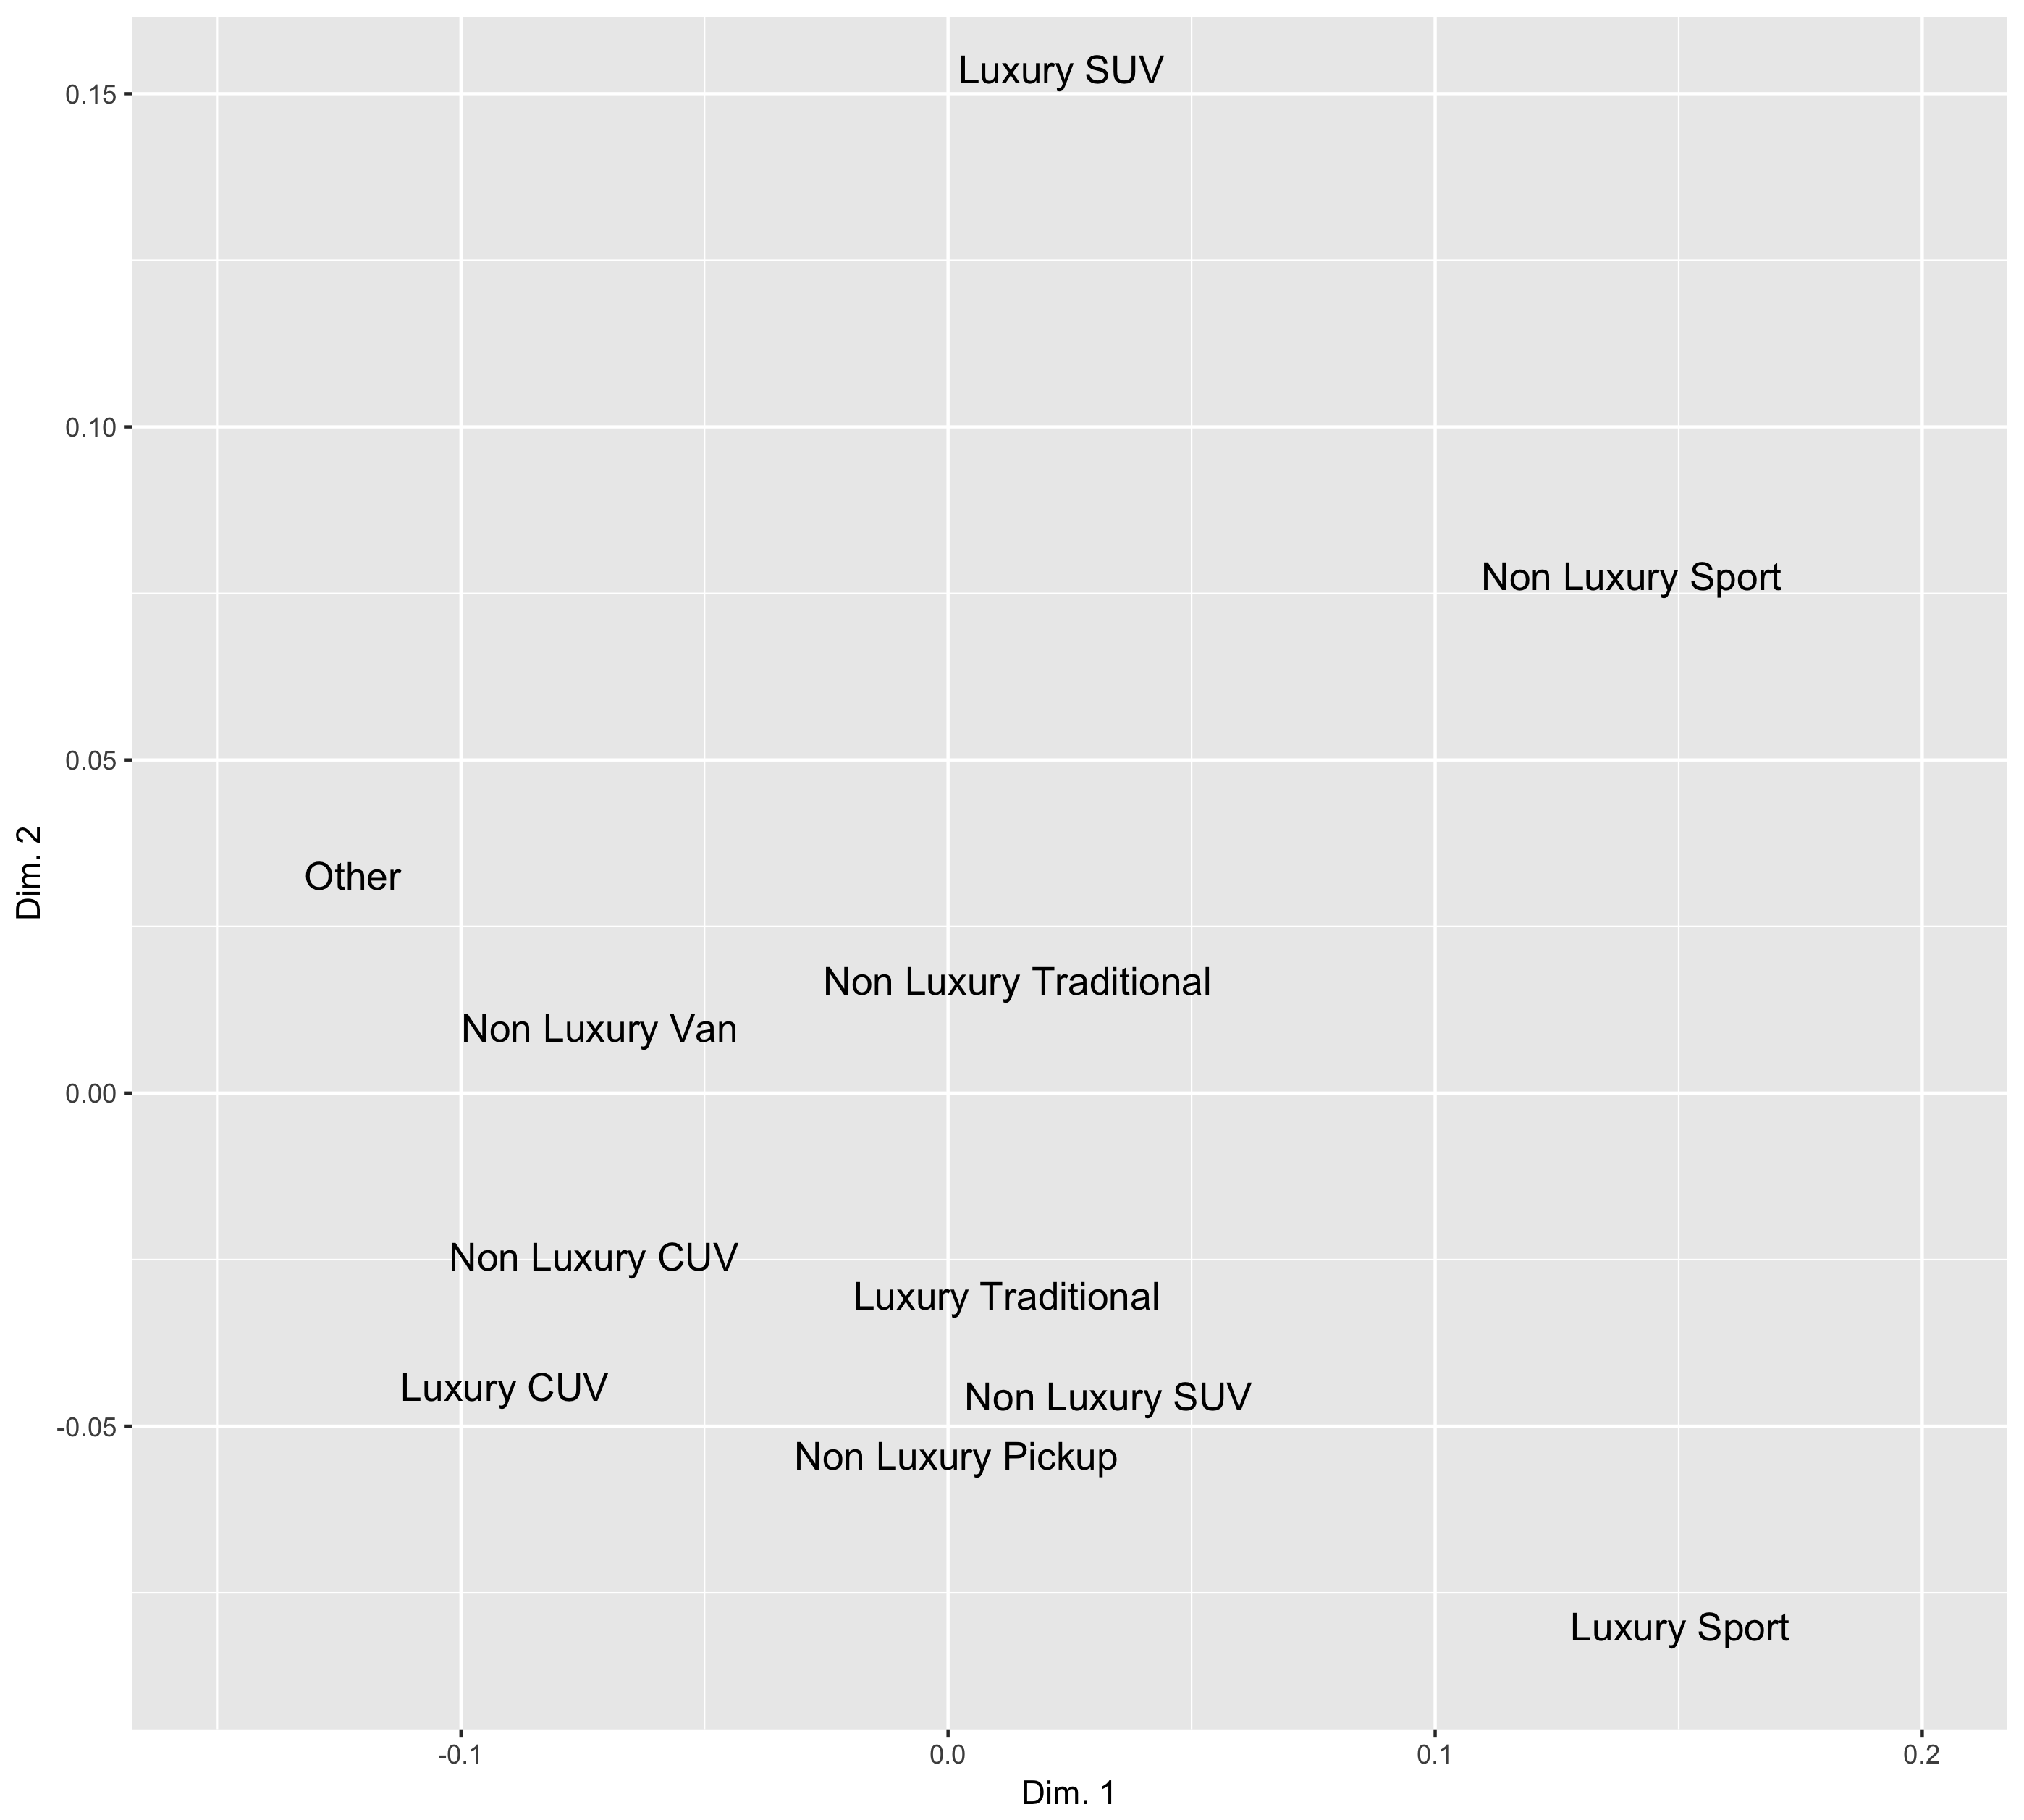
\includegraphics[width=1\linewidth]{VehicleTypeMDSPlot.png}
  \caption{Vehicle Type MDS}
  \label{fig:sub2}
\end{subfigure}
\caption{Multidimensional Scaling for Vehicle Manufacturer and Vehicle Type}
\label{fig:test}
\end{figure}

The plots don't indicate strong patterns of differentiation, but there are some noteworthy indicators. In particular, these results suggest the behavior of luxury sport/SUV drivers to be somewhat distinct, as noted by the outlying values for the BMW/Land Rover\footnote{Note that this analysis considers all Jaguar models to be part of Land Rover} in figure (a), and for Luxury SUV and Sport vehicles in figure (b).

To numerically explore this issue more fully, we draw on results of a logistic regression model (discussed more fully in the next section) to consider how a vehicle's manufacturer affects the likelihood of a multi-fatality collision.\footnote{Note again that the data here are drawn solely from accidents involving at least one fatality. Therefore, classification methods such as this are predicting the severity of an accident, \textit{given that one has already occurred.}}

\begin{table}[ht]
\centering
\begin{tabular}{rrl}
  \hline
 & Odds.Ratios & Automaker \\ 
  \hline
1 & 0.85 & Volkswagen \\ 
  2 & 0.70 & Honda \\ 
  3 & 0.62 & Mazda \\ 
  4 & 0.50 & Ford \\ 
  5 & 0.41 & Toyota \\ 
  6 & 0.39 & Volvo \\ 
  7 & 0.39 & FCA/Chrysler \\ 
  8 & 0.33 & GM \\ 
  9 & 0.27 & Hyundai-Kia \\ 
  10 & 0.21 & Mitsubishi \\ 
  11 & 0.10 & Daimler \\ 
  12 & 0.06 & Nissan \\ 
  13 & -0.07 & Subaru \\ 
  14 & -0.34 & Land Rover \\ 
   \hline
\end{tabular}
\caption{Automaker Odds Ratios for Predicting Multi-Fatality Accident (Relative to BMW)} 
\end{table}

\textbf{Automakers in the context of predicting multi-fatality incidents} \\
To explore this issue, we generated a binary 1-0 indicator for whether an incident involved more than 1 fatality, and tested the classification performance of a series of different models, the results of which are shown below. To overcome the class imbalance issue, we employ the resampling procedure employed by the SMOTE algorithm (for ``Synthetic Minority Over-sampling TEchnique"), developed by Chawla, et al. (2002). SMOTE uses a combination of over-sampling of the minority class and under-sampling of the majority to improve class balance. \\

The below table shows relative test error rates for classification using logistic regression, support vector machine, and adaptive boosting methods. \\

\begin{table}[ht]
\centering
\begin{tabular}{rrrr}
  \hline
 & Logistic Regression & Supp. Vec. Machine & AdaBoost \\ 
  \hline
Accuracy & 0.75 & 0.80 & 0.79 \\ 
   \hline
\end{tabular}
\caption{Test Set Prediction Accuracy} 
\end{table}

For interpreting the sign of a given predictor's relationship with the incidence of multi-fatality accidents, we leverage the logistic regression results, which allow for easier interpretation of estimated coefficients when compared to SVM and AdaBoost methods. The below table lists odds ratios for various predictors considered here.\footnote{Note that these results are obtained from the same logistic regression model described above containing the automaker odds ratio values}

\begin{table}[ht]
\centering
\begin{tabular}{rrl}
  \hline
 & OddsRatio & Variable \\ 
  \hline
1 & 0.26 & Distracted \\ 
  2 & 1.40 & On Drugs \\ 
  3 & 0.73 & No Restraint \\ 
  4 & 0.85 & Hit and Run \\ 
  5 & 0.66 & Speeding \\ 
  6 & -0.29 & Previous Recorded Crashes \\ 
  7 & -0.33 & Previous DWI Convictions \\ 
  8 & -0.04 & Previous Recorded Suspensions And Revocations \\ 
  9 & 0.01 & Travel Speed \\ 
  10 & 0.66 & Drunk \\ 
  11 & 0.68 & Inclement Weather \\ 
  12 & 0.44 & Intersection \\ 
  13 & -0.00 & Hour of Crash \\ 
   \hline
\end{tabular}
\caption{Predictor Odds Ratios} 
\end{table}

Finally, to assess the actual significance of automaker within the context of other predictors, we reference the below output, which illustrates variable importance rankings for the SVM and AdaBoost classifiers. The models don't completely agree on relative variable importance, but there are some key patterns. For example, key for both models is the fact that the hour of crash is a dominant predictor of the likelihood a fatal accident resulted in multiple deaths. In addition, a driver's record, potential drug use, and driving speed are especially significant for predicting multi-fatality accidents. Interestingly, whether or not a driver was distracted (using a cellphone, for example), and whether the weather was clear or not, appear to be relatively less significant determinants of the likelihood that a fatal accident involved multiple deaths. Further assessment of this question would consider the affect of these less important predictors on non-fatal accidents, as well as fatal ones. Finally, this analysis suggests that, within the context of other fatality-relevant predictors, automaker is relatively unimportant. Accounting for various driver behaviors has captured much of the meaningful variation in the outcome. \\

\begin{figure}[H]
\centering
  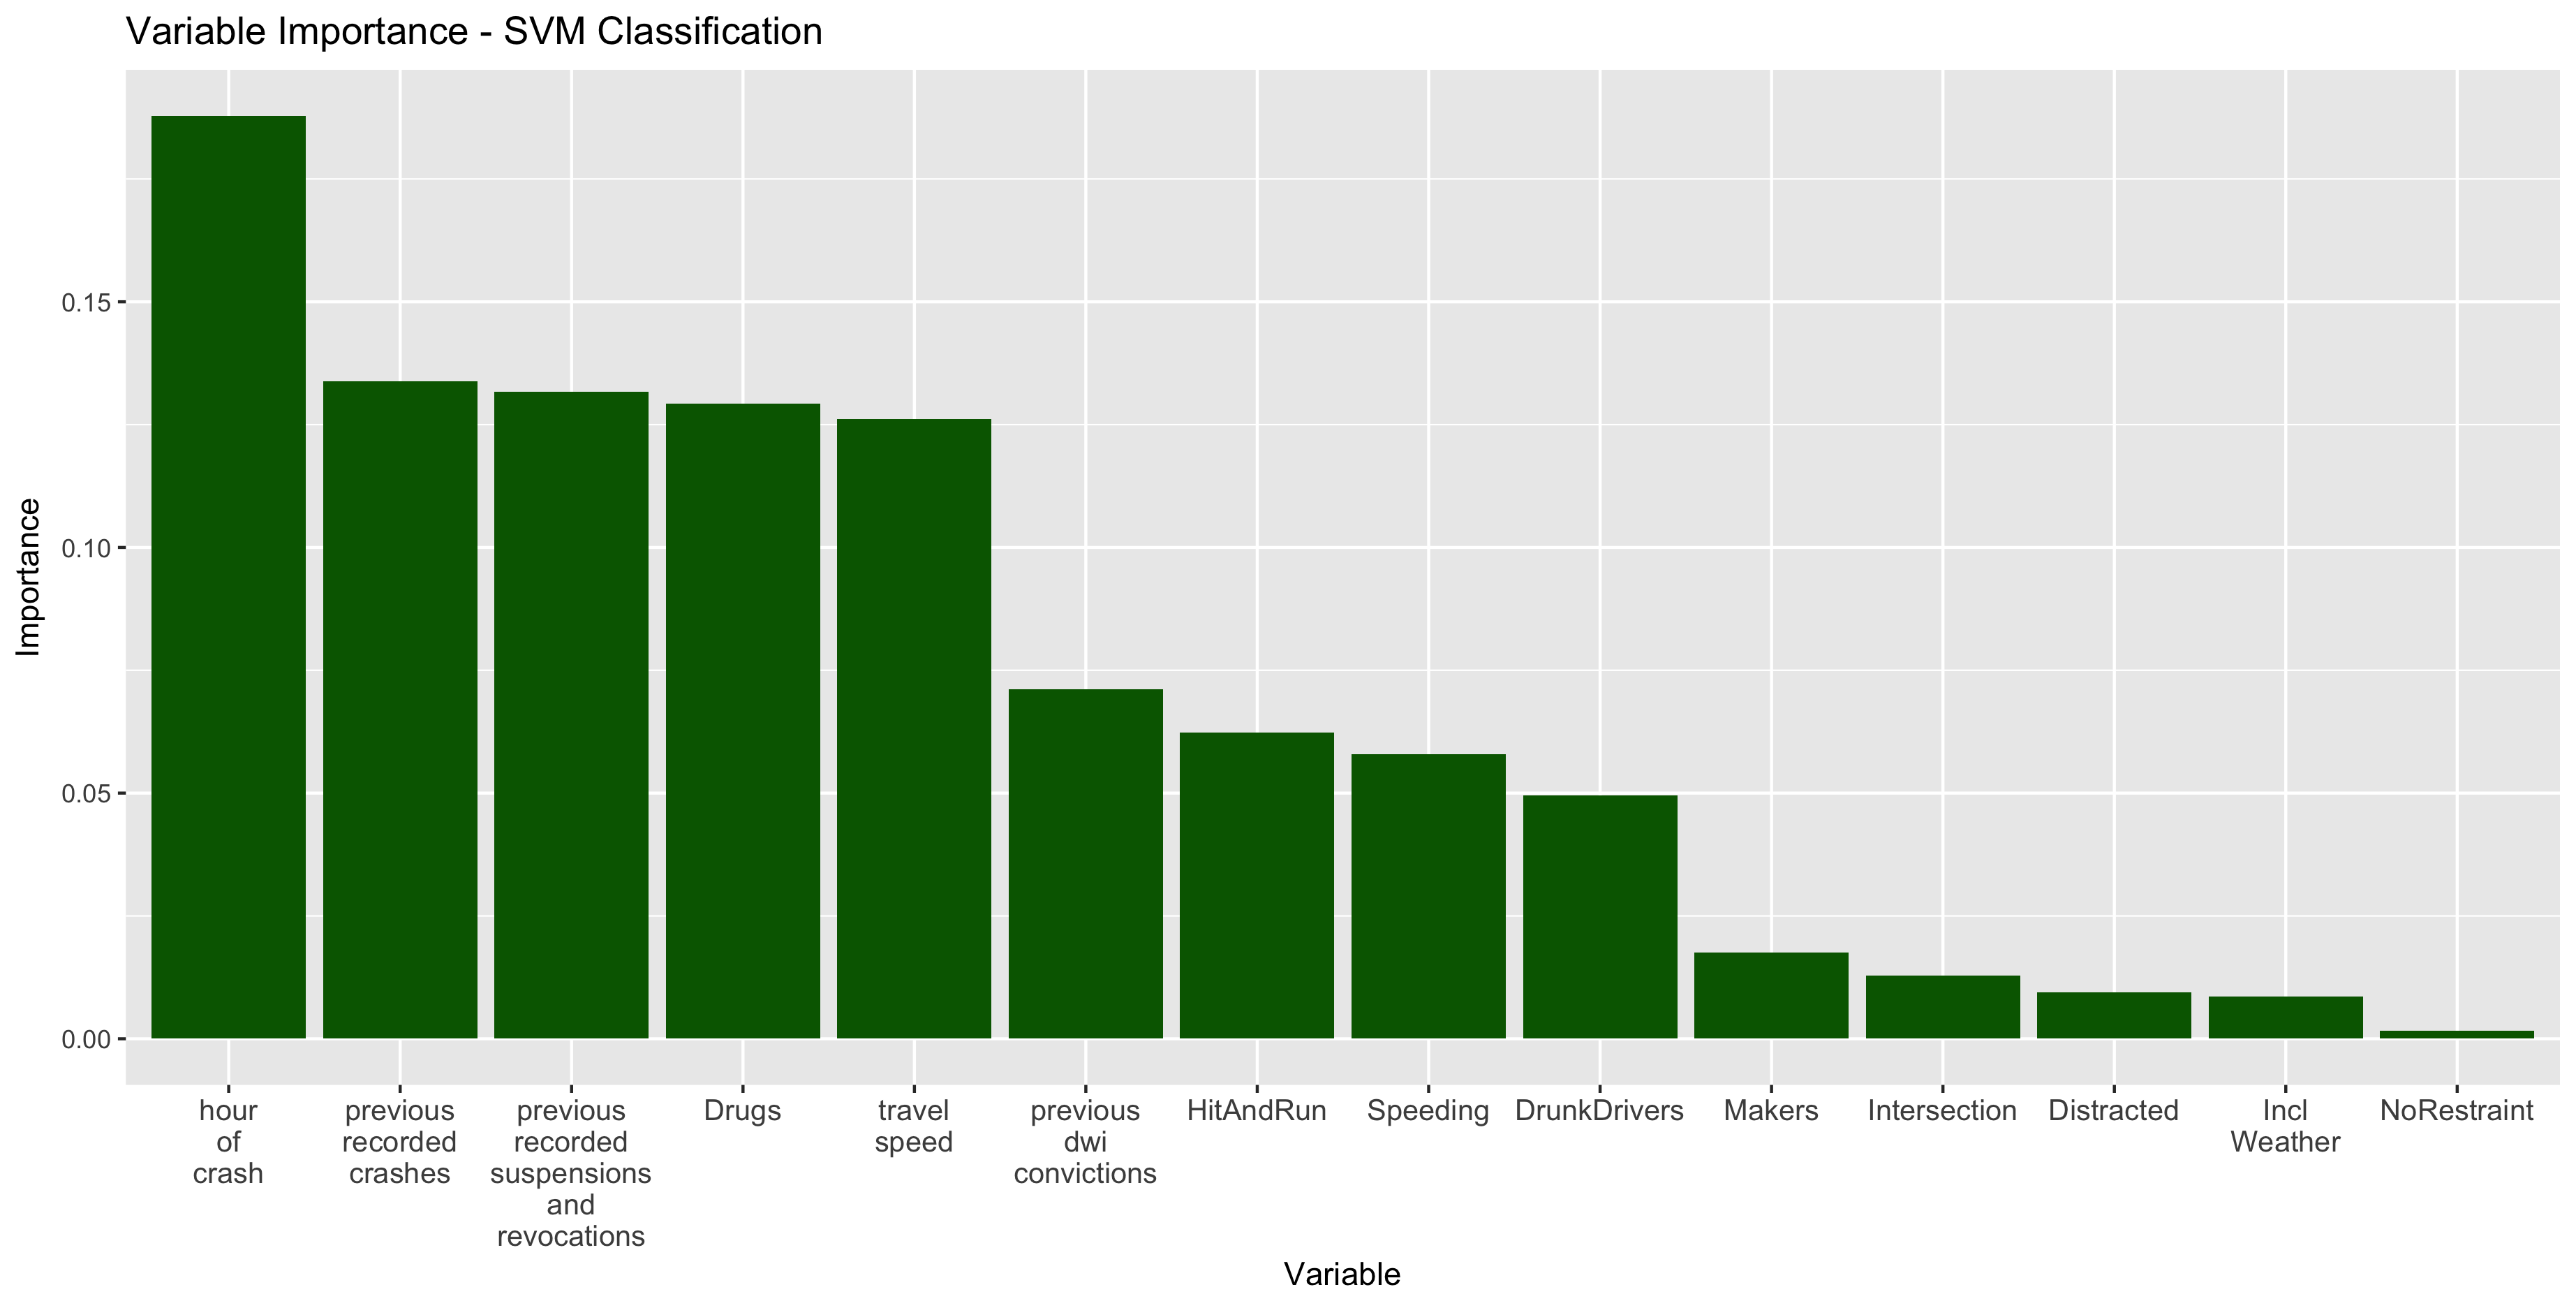
\includegraphics[width=15cm,height=8cm,keepaspectratio]{ImportancePlot_SVM.png}
\caption{Variable Importance - Support Vector Machine}
\end{figure}

\begin{figure}[H]
\centering
  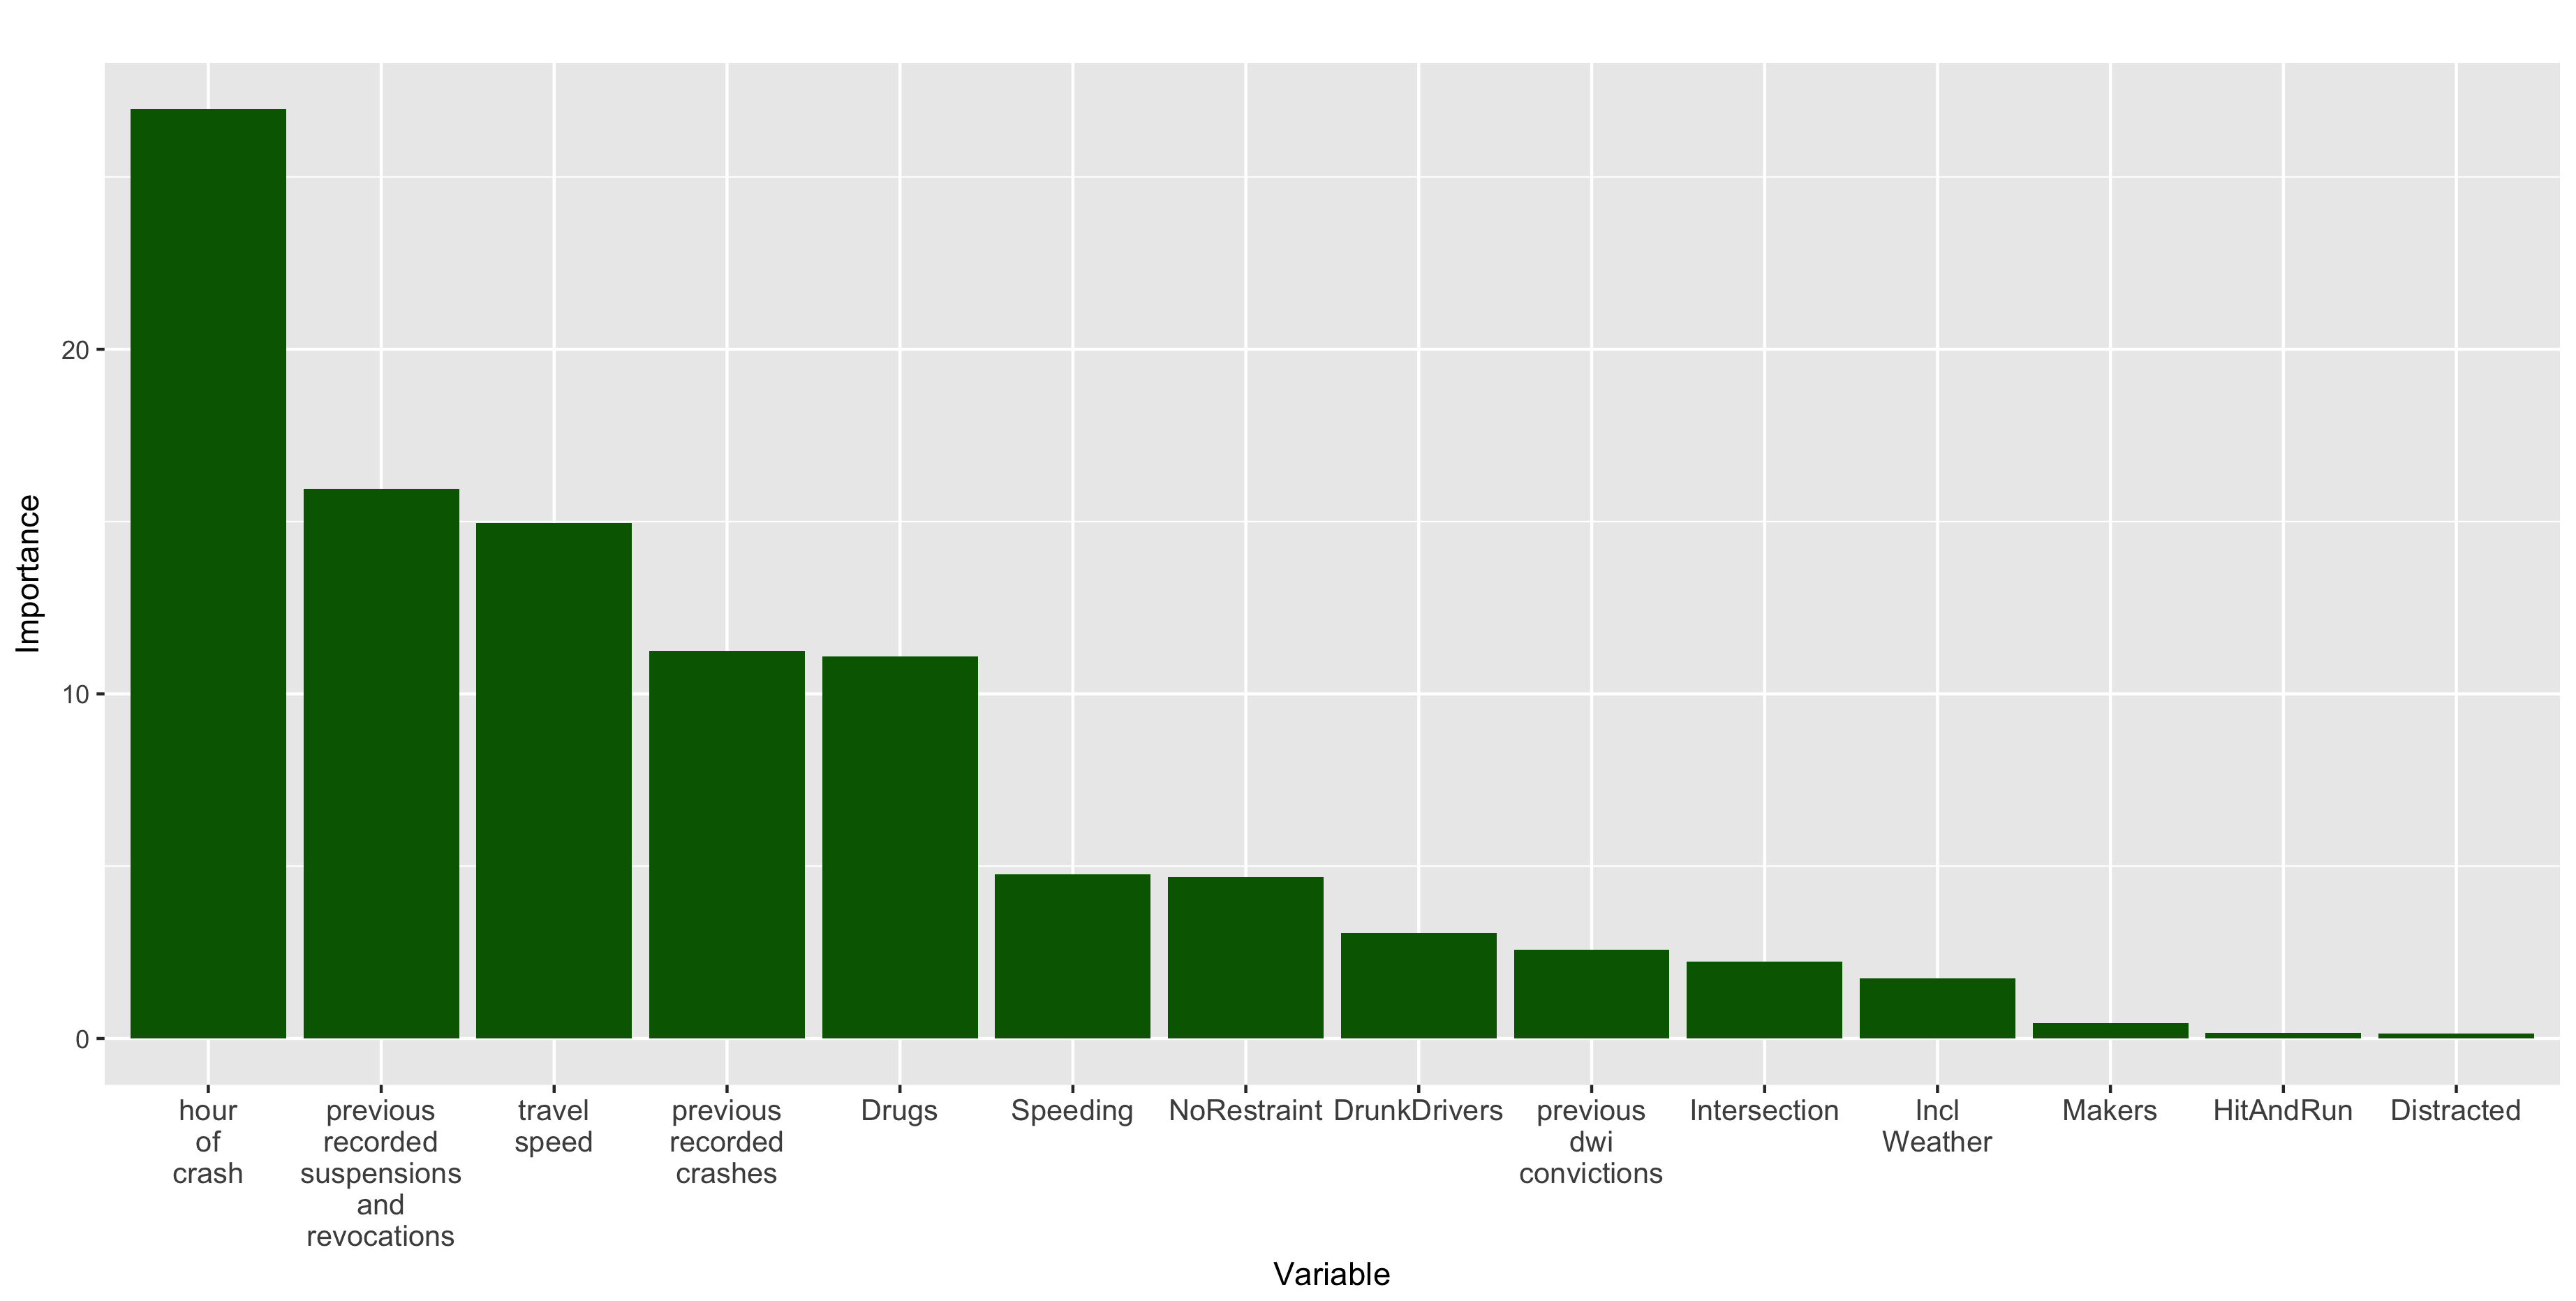
\includegraphics[width=15cm,height=8cm,keepaspectratio]{ImportancePlot_ADABoost.png}
\caption{Variable Importance - AdaBoost Algorithm}
\end{figure}

The below two sections explore in further detail the issues of driver impairment and hit and run incidents.

\section*{Driver Impairment}

(Teerth Insert Analysis Here)

\section*{Hit-and-Run}

According to an NHTSA report in 2014, nearly one in five pedestrians killed were involved in hit-and-run crashes. In this section we will discuss hit-and-run behavior as it brings more risk of fatalities during traffic accident. We are interested in what characteristics are more correlated with hit-and-run. We generated a binary of 1 when there is hit-and-run and 0 otherwise. Since the focus is on inference rather than prediction, we used logistic regression, where hit-and-run as dependent variables and representative driver behavior and natural features such as spending, past driving history and time of the accident are used as independent variables. With some model selection, we get the following regression result.  

\begin{table}[!htbp] \centering 
	\caption{} 
	\label{} 
	\begin{tabular}{@{\extracolsep{5pt}}lc} 
		\\[-1.8ex]\hline 
		\hline \\[-1.8ex] 
		& \multicolumn{1}{c}{\textit{Dependent variable:}} \\ 
		\cline{2-2} 
		\\[-1.8ex] & HitAndRun \\ 
		\hline \\[-1.8ex] 
		Distracted & 0.216$^{***}$ (0.025) \\ 
		Drugs & 0.307$^{***}$ (0.048) \\ 
		MultiFatality & $-$1.059$^{***}$ (0.050) \\ 
		Speeding & 1.018$^{***}$ (0.029) \\ 
		previous\_recorded\_crashes & 0.004 (0.020) \\ 
		previous\_dwi\_convictions & 0.777$^{***}$ (0.040) \\ 
		previous\_recorded\_suspensions\_and\_revocations & 0.158$^{***}$ (0.007) \\ 
		DrunkDrivers & 0.110$^{***}$ (0.028) \\ 
		daytime & $-$0.816$^{***}$ (0.032) \\ 
		evening & 0.153$^{***}$ (0.031) \\ 
		Constant & $-$1.270$^{***}$ (0.030) \\  
		\hline \\[-1.8ex] 
		\textit{Note:} Standard error is in bracket & \multicolumn{1}{r}{$^{*}$p$<$0.1; $^{**}$p$<$0.05; $^{***}$p$<$0.01} \\ 
	\end{tabular} 
\end{table} 

According to the table, speeding, previous DWI convictions and drugs are highly correlated with an increase in hit-and-runs. There is also a significant reduction in probability of hit-and-runs during the daytime (7am to 6pm) than night and evening. Other risk factors are also associated with higher chances of hit-and-run. 

The most surprising finding is that the indicator of multiple fatalities has a significantly negative coefficient. We believe there is a possibility of confounding variables. For example, hit-and-run crashes mostly involve pedestrians and likely to have single fatality. In addition, a multiple-fatality crash might mean a severe crash that the drivers may not even survive to commit hit-and-runs. With these two potential confounding variables, it is possible for multiple-fatality to have a negative coefficient.  


\section*{Environmental Factors}
A proper analysis of environmental factors is both beyond the scope of this analysis, and requires incorporating a richer set of weather data than the handful of indicators available in the FARS system. A quick initial check of the relevance of environmental conditions doesn't return many relevant results. The plot below shows data from Cook County, Illinois, chosen for its high number of traffic fatalities and variable weather\footnote{Especially when compared to Dallas, Phoenix, and LA County}. The vast majority of fatal collisions occur in clear weather, which is due in large part no doubt to the fact that it is simply clear much more often in Chicago than it is rainy or snowy! 

\begin{figure}[H]
\centering
  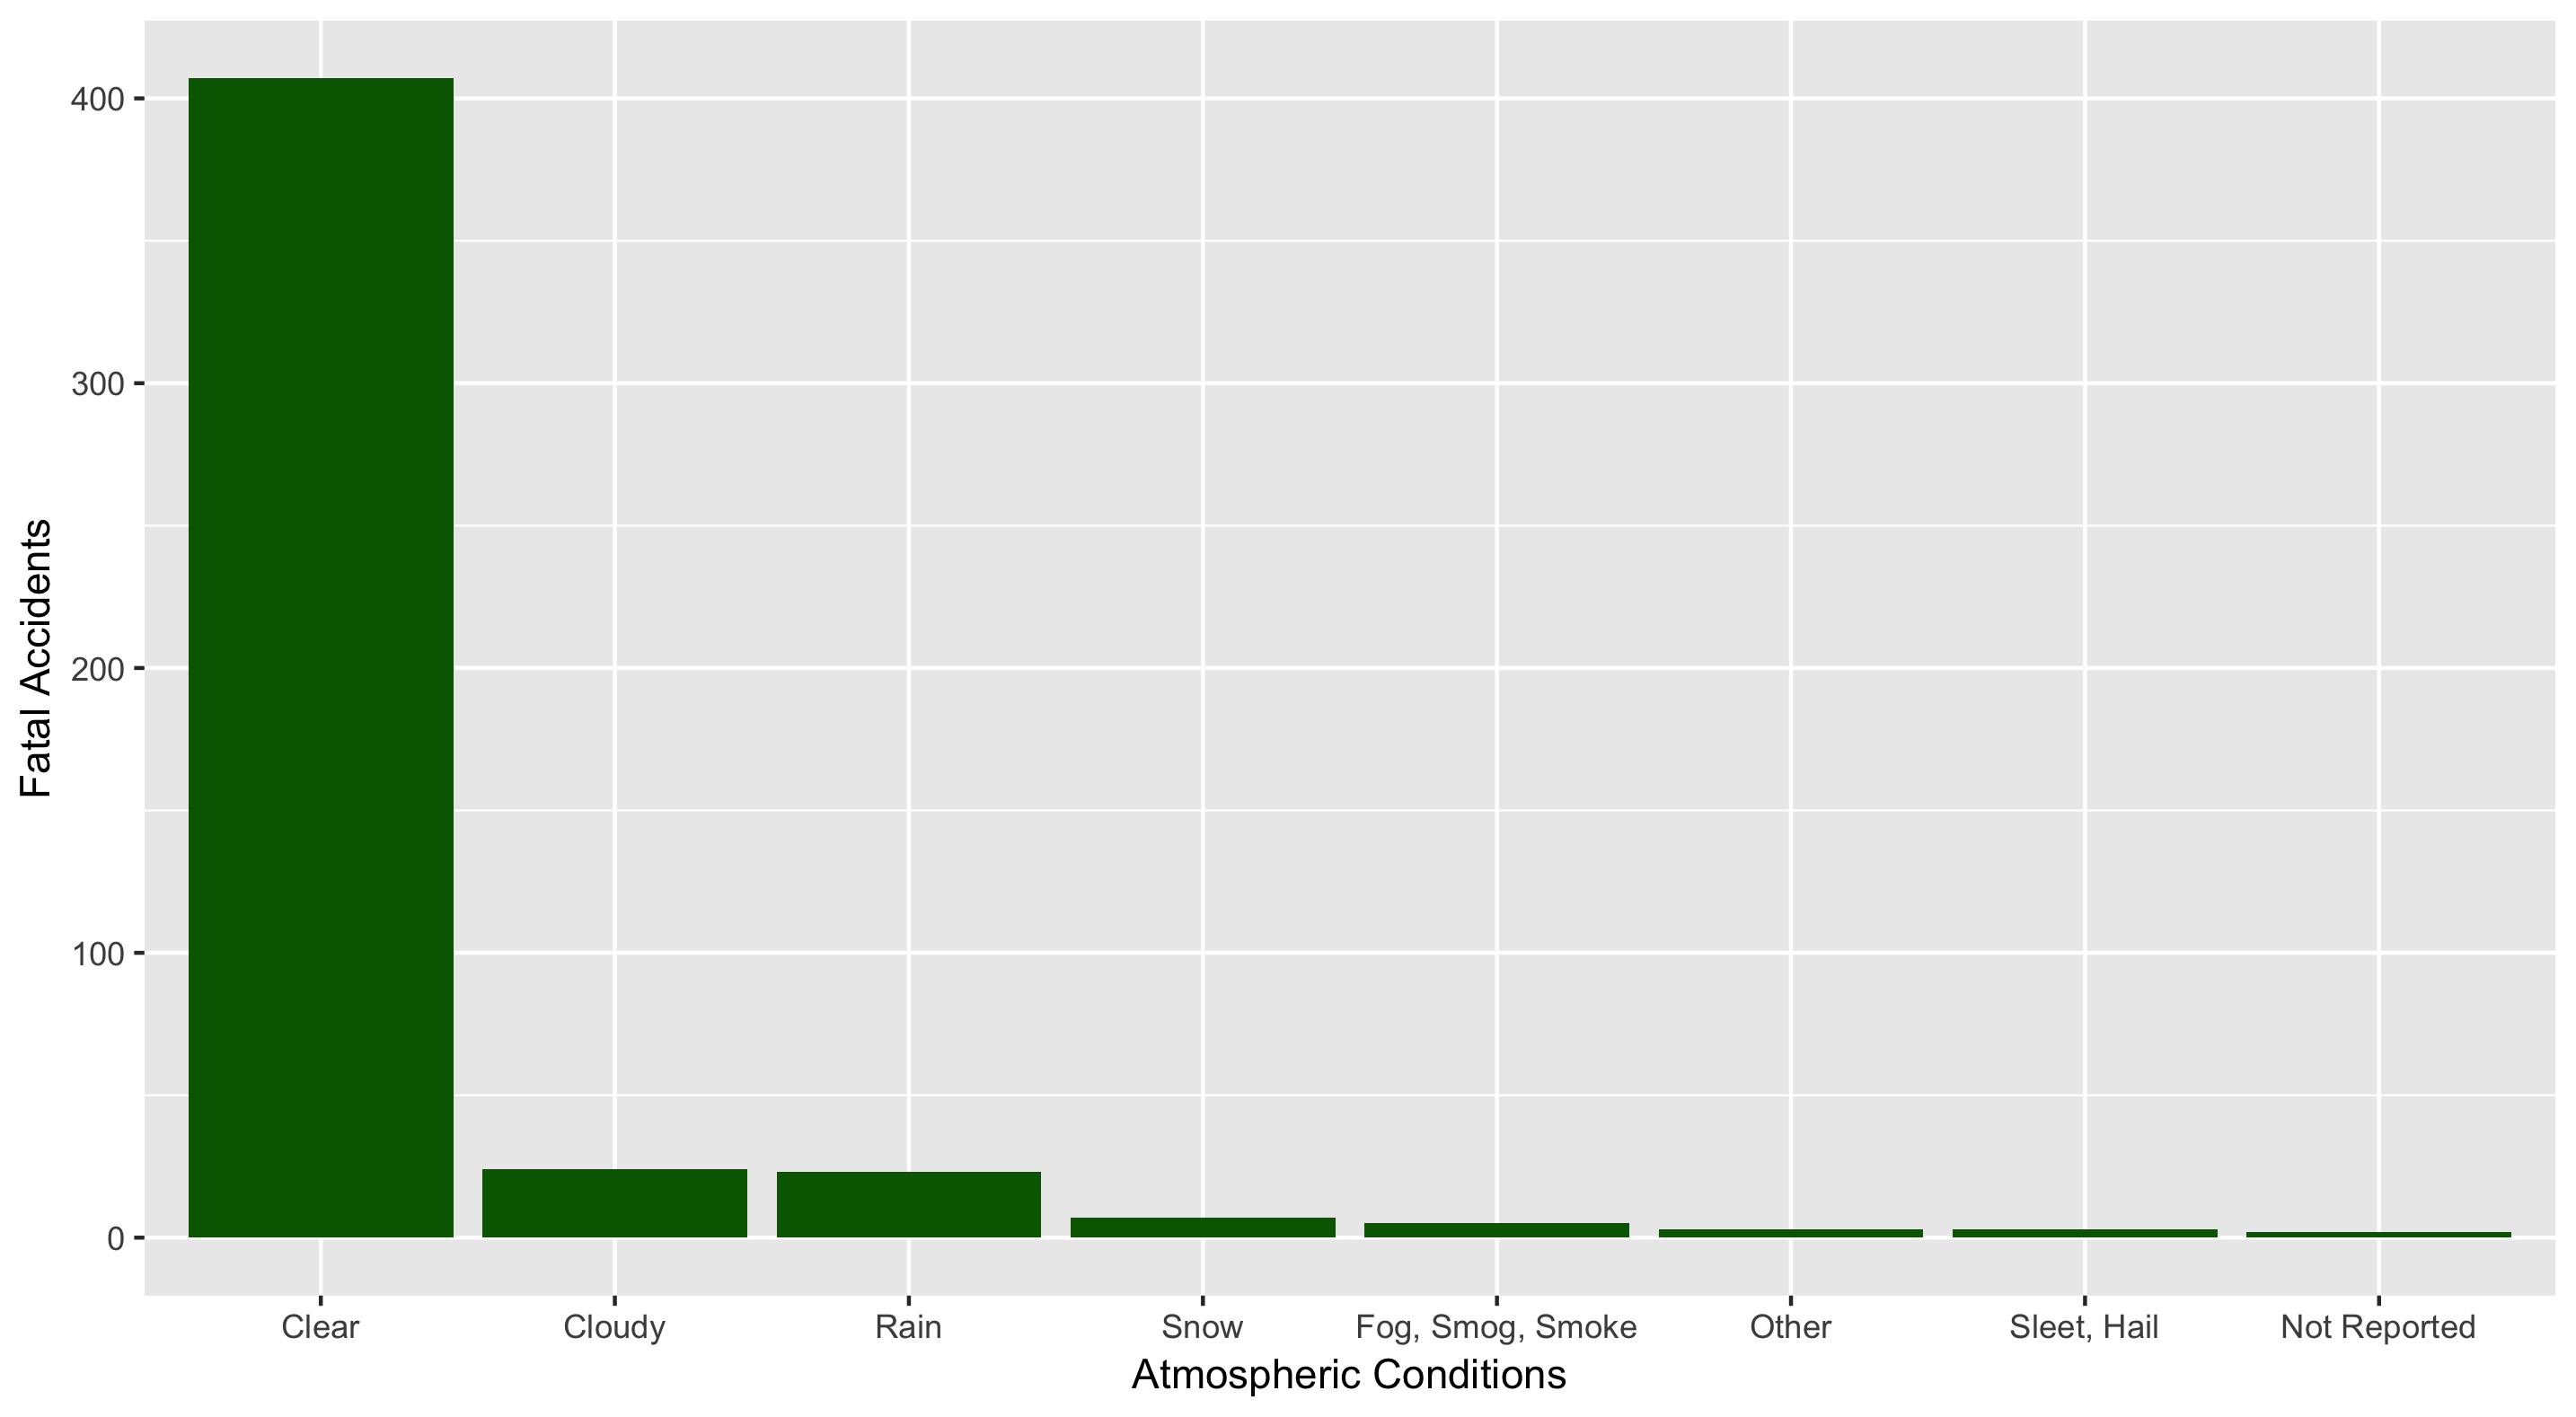
\includegraphics[width=15cm,height=8cm,keepaspectratio]{Environmental.png}
\caption{Fatal Accidents in Cook County, by Atmospheric Condition}
\end{figure}


\section*{Conclusion}

(To be updated once final analyses incorporated)


\section*{References}
\begin{hangparas}{1.27cm}{1}
Batterman, Stuart, Richard Cook, and Thomas Justin. ``Temporal variation of traffic on highways and the development of accurate temporal allocation factors for air pollution analyses." \textit{Atmos Environ}. Apr. 2015.

Chawla, Nitesh, Kevin Bowyer, Lawrence Hall, and W. Philip Kegelmeyer. "SMOTE: Synthetic Minority Over-sampling Technique." \textit{Journal of Artificial Intelligence Research}. 2002.

Choi, Eun-Ha. ``Crash Factors in Intersection-Related Crashes: An On-Scene Perspective." \textit{U.S. Department of Transportation - National Highway Traffic Safety Administration}. Sept. 2010.

Gravano, Luis and John Paparrizos. ``k-Shape: Efficient and Accurate Clustering of Time Series." \textit{SIGMOD}. June 2015.

Zador, P.L, S.A. Krawchuk, and R.B. Voas. ``Relative Risk of Fatal Crash Involvement by BAC, Age, and Gender." \textit{U.S. Department of Transportation - National Highway Traffic Safety Administration}. Apr. 2000.

``National Motor Vehicle Crash Causation Survey: Report to Congress." \textit{U.S. Department of Transportation - National Highway Traffic Safety Administration}. July 2008.

``2014 Traffic Safety Factsheet Pedestrians." \textit{U.S. Department of Transportation - National Highway Traffic Safety Administration}. May 2016.

\end{hangparas}




\end{document}  
